\documentclass{report}

%% Set up the bibliography
\usepackage[style=authoryear]{biblatex}
\addbibresource{references.bib}

\usepackage{lipsum}

%% Index

%\usepackage{imakeidx}
%\makeindex[columns=2]


\usepackage{glossaries}
\makeglossaries



%% Additional packages and commands
%\setlist{itemsep=-2pt} % Reducing white space in lists slightly
\renewcommand{\deg}{\si{\degree}\xspace} % Use \deg easily, everywhere

\renewcommand{\listfigurename}{Liste des illustrations}
\renewcommand{\listtablename}{Liste des tableaux}

\usepackage{xcolor}
\usepackage{mdframed}
\usepackage{newfloat}

% Définition d'un nouvel environnement pour les encarts méthodologiques
\DeclareFloatingEnvironment[fileext=frm,placement={!ht},name=Encart]{method}
%\captionsetup[method]{labelfont=bf}

% Couleur de fond pour les encarts
%\definecolor{lightgray}{RGB}{240,240,240}

% Définition du style des encarts
\mdfdefinestyle{methodstyle}{
    backgroundcolor=lightgray,
    linewidth=0pt,
    roundcorner=5pt,
    innertopmargin=10pt,
    innerbottommargin=10pt,
    innerleftmargin=10pt,
    innerrightmargin=10pt
}



\newcommand{\methodtitle}[1]{%
    \refstepcounter{method}%
    \textbf{Méthode \arabic{method} : #1} \\
    \par
}

% Définition de l'environnement "methodbox"
\newenvironment{methodbox}[1][]
{\begin{mdframed}[style=methodstyle]\methodtitle{#1}\ignorespaces}
{\end{mdframed}}


%% ----------------------------------------------------------------------
%%    Begin of document + Frontmatter (Roman page numbering)
%% ----------------------------------------------------------------------

\linespread{1.15}



\begin{document}




\newglossaryentry{tipping point}
{
    name=tipping point, 
    plural = tipping points, 
    description={Un \textit{tipping point} est un point où la dynamique du système change.}
}

\newglossaryentry{risk tipping point}
{
    name=risk tipping point,
    plural = risk tipping points, 
    description={}
}

\newglossaryentry{regime climatique}
{
    name=régime climatique, 
    description={Terme repris de \cite{aykut_gouverner_nodate}, qui le décrivent comme un \enquote{système complexe d’arènes et d’institutions qui a réuni des acteurs et des partenaires de plus en plus nombreux, a suscité de nouvelles pratiques de recherche, a instauré des procédures d’évaluation et de validation, a vu s’affronter des intérêts économiques et des enjeux politiques variés et a établi, enfin, des relations particulières entre sciences, expertise, politiques et marchés}.}
}

\newglossaryentry{cout social du carbone}
{
    name=coût social du carbone, 
    description={Un modèle est une représentation simplifiée de la réalité, qui permet de la rendre intelligible. C'est le produit de la modélisation, \textit{l'élément du dispositif scientifique qui fait médiation entre le système réel et la théorie} \cite{briens_decroissance_2015}. Il y en a deux types : des modèles appliqués et quantitatifs, et des modèles théoriques plus stylisés \cite{briens_decroissance_2015}. Le rôle central des modélisateur.ices dans la fabrication du modèle est souvent mis en avant, comme par exemple chez \cite{beck_epistemic_2016} : \textit{model building is an art and not a mechanical procedure}. \\}
}


\newglossaryentry{modele}
{
    name=modèle, 
    plural = modèles, 
    description={Un modèle est une représentation simplifiée de la réalité, qui permet de la rendre intelligible. C'est le produit de la modélisation, \textit{l'élément du dispositif scientifique qui fait médiation entre le système réel et la théorie} \cite{briens_decroissance_2015}. Il y en a deux types : des modèles appliqués et quantitatifs, et des modèles théoriques plus stylisés \cite{briens_decroissance_2015}. Le rôle central des modélisateur.ices dans la fabrication du modèle est souvent mis en avant, comme par exemple chez \cite{beck_epistemic_2016} : \textit{model building is an art and not a mechanical procedure}. \\}
}

\newglossaryentry{modelisation}
{
    name=modélisation, 
    plural = modélisation, 
    description={La modélisation est une pratique visant à produire un \gls{modele}.}
}

\newglossaryentry{iam}
{
    parent=modele,
    name=modèle intégré, 
    plural = modèles intégrés, 
    description={Les modèles intégrés sont des \textit{représentations simplifiées de systèmes sociaux et physiques complexes, qui se concentrent sur les interactions entre l'économie, la société et l'environnement} \cite{intergovernmental_panel_on_climate_change_ipcc_annex_2023}  \\
    On peut distinguer deux grandes familles de modèles intégrés : les modèles de \textit{policy optimization} et ceux de \textit{policy evaluation}. Les premiers visent à trouver le "meilleur" chemin parmis toutes les options possibles, c'est à dire celui maximisant une fonction objectif. Les seconds permetent de voir l'évolution de variables clés au fil du temps, mais ne vise pas à maximiser des variables. \\
    Malgrè de nombreuses limites, ils constituent un outil essentiel de la prise de décision climatique.
    }
}

\newglossaryentry{damage function}
{
    name=fonction de dommage, 
    plural = fonctions de dommage, 
    description={Composant du modèle permettant de représenter les dommages du changement climatique. Plus précisement, Waidelich et al \cite{waidelich_climate_2024} les définissent comme \emph{projections of economic damage from climate change are key for evaluating climate mitigation benefits, identifying effects on vulnerable communities and informing discussions around adaptation needs, as well as loss and damage financing.}}
}

\newglossaryentry{scenario}
{
    name=scénario,
    plural = scénarii, 
    description={Un scénario est une jeu de paramètre que l'on donne à un modèle}
}

\newglossaryentry{imp}
{
    name=illustrative mitigation pathways, 
    description={Trajectoires d'atténuation stéréotypée}
}

\newglossaryentry{attenuation}
{
    name=atténuation, 
    description={Réduction de l'ampleur du changement climatique par la réduction des émissions de gaz à effet de serre}
}


\newglossaryentry{ethique}
{
    name=éthique, 
    description={}
}

\newglossaryentry{procedural ethics}
{
    name=éthique procédurale, 
    description={Respect des lignes conductrices et des usages dans un travail de recherche. Correspond à ce que l'on appelle communément de la \textit{bonne recherche} (good science). \cite{tuana_leading_2010} la définit ainsi : \enquote{ethical aspects of the process of conducting scientific research, such as: falsification, fabrication, and plagiarism; care for subjects (human and non-human animal); responsible authorship issues; analysis of and care for data}.}
}

\newglossaryentry{intrinsic ethics}
{
    name= éthique intrinsèque, 
    description={Valeurs personnelles qui sont incorporées dans le travail de recherche, de manière consciente ou non. \cite{tuana_leading_2010} la définit ainsi : \enquote{ethical issues and values that are embedded in or otherwise internal to the production of scientific research and analysis. These involve ethical issues arising from, for example: the choice of certain equations, constants, and variables; analysis of data; handling of error, and degree of confidence in projections.}}
}

\newglossaryentry{extrinsic ethics}
{
    name=éthique extrinsèque, 
    description={Dimension éthique des effets que produit la recherche sur la société. \cite{tuana_leading_2010} la définit ainsi : \enquote{ethical issues that are external to the production of scientific research. These arise, for example, when considering the impact of scientific research on society; e.g., the effects of technological innovations on social ends such as health and well-being, whether pressing social and economic issues are likely to be addressed and if so, who benefits, and the role of science in policy-making.}}
}

\newglossaryentry{incertitude}
{
    name=incertitude, 
    plural = incertitudes, 
    description={Selon le Larousse, désigne les \emph{points, éléments qui, dans quelque chose, ne peuvent être connus à l'avance, sont imprévisibles}. Peut être lié soit à un déficit d'information, à un \emph{manque de données}, soit à de l'indetermination. Ainsi, Walker et al., cité par \cite{beck_epistemic_2016}, la décrit comme \enquote{any departure from the unachievable ideal of complete determinism}. Toujours selon eux, l'incertitute dans les modèles intégrés existe sous deux formes : l'incertitude scientifique, qui désigne les limites (actuelles à la connaissance), sur les causes, processus et conséquences du changement climatique; et l'incertitude éthique, qui désigne l'absence de consensus sur le cadre éthique adéquat.}
}

\newacronym{SCC}{SCC}{social cost of carbon}

\newacronym{FUND}{FUND}{Climate Framework for Uncertainty, Negotiation and Distribution model}

\newacronym{DICE}{DICE}{Dynamic Integrated Climate-Economy model}

\newacronym{PAGE}{PAGE}{Policy Analysis of Greenhouse Effect model}

\newacronym{CCNUCC}{CCNUCC}{Convention Cadre des Nations Unies sur le Changement Climatique}

\newacronym{SBSTA}{SBSTA}{Subsidiary Body on Science and Technical Advice}

\newacronym{COP}{COP}{Conference Of Parties}

\newacronym{ipcc}{IPCC}{Voir GIEC}

\newacronym{AR6}{AR6}{Sixth Assesment Report}

\newacronym{WILIAM}{WILIAM}{WIthin Limits Integrated Assesment Model}

\newacronym{GIEC}{GIEC}{Groupe Intergouvernemental d'Experts sur le Climat. Il s'agit dun groupe d'experts, qui travaillent pour faire la synthèse des connaissances disponibles en matière de climat. \cite{cointe_ar6_2024}}




%\frontmatter

%% Define the main parameters
\title{Fonctions de dommages dans les modèles intégrés}
%\subtitle{Quelle forme, étendus et enjeux pour les fonctions de dommage ?}
\author{Gabriel Genelot}

%\subject{\textit{Mémoire de recherche}} % Cover only
%\affiliation{} % Cover only
%\coverimage{} % Aspect ratio of 2:3 (portrait) recommended
%\definecolor{title}{HTML}{A9CA53} % Color for cover title

%\makecover

\begin{titlepage}

\begin{center}

%% Print the title
{\makeatletter
\largetitlestyle\fontsize{45}{45}\selectfont\@title
\makeatother}

%% Print the subtitle
{\makeatletter
\ifdefvoid{\@subtitle}{}{\bigskip\titlestyle\fontsize{20}{20}\selectfont\@subtitle}
\makeatother}


\bigskip
\bigskip

%% Print the name of the author
{\makeatletter
\largetitlestyle\fontsize{25}{25}\selectfont\@author
\makeatother}

\bigskip

\href{mailto:gabriel.genelot@ens.psl.eu}{gabriel.genelot@ens.psl.eu}

\bigskip
\bigskip

%% Print table with names and student numbers
%\setlength\extrarowheight{2pt}
%\begin{tabular}{lc}
%    Student Name & Student Number \\\midrule
%    First Surname & 123456 \\
%\end{tabular}

\vfill

\textbf{Résumé} \\

\begin{center}
\justify


Nous explorons les enjeux éthiques liés à la modélisation des impacts du changement climatique. Dans un premier temps, nous recensons des fonctions de dommages issues de différents modèles, pour en comparer les caractéristiques et identifier des enjeux éthiques. Nous implémentons ensuite les fonctions de dommage de DICE, FUND et WITNESS au sein du modèle WILIAM, et proposons un coefficient qui représente l'équité spatiale. Nous abordons l'épistémologie des modèles intégrés au regard de ce nouveau coefficient, avant de de réaliser des entretiens semi-directifs avec des acteurs du régime climatique (chercheurs, décideurs). Nous montrons que les fonctions de dommage sont très sensibles aux implications éthiques sous-jacentes, et qu'il faut que celles soit explicitées et modifiables par les utilisateurs. 

\end{center}


\bigskip

\bigskip

%% Print some more information at the bottom
\begin{tabular}{lp{10cm}}
    Directrice : & Nadia Maïzi \\
    Tuteur : &  Thibaut Feix\\
    Cadre : & Mémoire de recherche de M2 \\
    Faculté : & Institut d'études du développement de la Sorbonne (IEDES), Université Paris 1 - Panthéon Sorbonne
\end{tabular}

\bigskip
\bigskip

%% Add a source and description for the cover and optional attribution for the template
\begin{tabular}{p{15mm}p{10cm}}
    %Couverture : & Photo by Tom Fisk from \href{https://www.pexels.com/photo/green-forest-2739664/}{Pexels}  \\
    % Feel free to remove the following attribution, it is not required - still appreciated :-)
    %Style: & EPFL Report Style, with modifications by Batuhan Faik Derinbay
\end{tabular}

\end{center}

%% Insert the EPFL logo at the bottom of the page
\begin{tikzpicture}[remember picture, overlay]
    \node[above=10mm] at (current page.south) {%
         
\includegraphics[width=0.5\linewidth]{figures/logos/iedes_logo.jpg}
    };
\end{tikzpicture}

\end{titlepage}

\chapter*{Remerciements}
\addcontentsline{toc}{chapter}{Remerciements}

\emph{A preface...}

\begin{flushright}
{\makeatletter\itshape
    \@author \\
    Paris, septembre 2024
\makeatother}
\end{flushright}

\chapter*{Summary}
\addcontentsline{toc}{chapter}{Summary}

\emph{A summary...}


\tableofcontents

coucou tout le monde 


%\chapter*{Nomenclature}
\addcontentsline{toc}{chapter}{Nomenclature}

\emph{If a nomenclature is required, a simple template can be found below for convenience. Feel free to use, adapt or completely remove.}

\section*{Abbreviations}

\begin{longtable}{p{2.5cm}p{8cm}}
    \toprule
    Abbreviation & Definition \\
    \midrule\endhead % Add abbreviations alphabetically here:
    ISA & International Standard Atmosphere \\
    ... \\
    \bottomrule
\end{longtable}

\section*{Symbols}

\begin{longtable}{p{2.5cm}p{8cm}p{2.5cm}}
    \toprule
    Symbol & Definition & Unit \\
    \midrule\endhead % Add Latin symbols alphabetically here:
    $V$ & Velocity & [m/s] \\
    ... \\
    \midrule % Add Greek symbols alphabetically here:
    $\rho$ & Density & [kg/m$^3$] \\
    ... \\
    \bottomrule
\end{longtable}


%% ----------------------------------------------------------------------
%%    Mainmatter (Arabic page numbering)
%% ----------------------------------------------------------------------

%\mainmatter



\PEEL{Les modèles intégrés sont sensibles aux choix éthiques des modélisateur.ices, ce qui a des conséquences importantes sur leur rôle dans la société.}{Taux d'actualisation, inégalités}{La prise en compte des inégalités (spatiales, sociales, temporelles) est un facteur majeur du niveau de dommage; la manière de les prendre en compte résulte de choix éthiques.}{On doit donc avoir un regard critique sur ces différents choix. }




\chapter*{Introduction}
\newrefsegment

\PEEL{Exposez l'idée principale ou l'argument que vous souhaitez développer dans cette partie.}{Fournissez des preuves, des données ou des citations qui soutiennent votre point.}{Expliquez en quoi les preuves que vous avez fournies sont pertinentes et comment elles appuient votre point.}{Faites le lien avec le sujet principal ou avec la section suivante de votre mémoire.}


%% Amorce

% réduction de l'incertitude => elle est désagréable donc on cherche toujours à la minimiser; 
% representer le monde le plus précisement possible => fantasme et ambition des sciences => La carte et le navigateur \cite{edenhofer_mapmakers_2014}. 



% Comment prendre les bonnes décisions face au changement climatique ? 



Longtemps, l'emphase a été mise sur la production de connaissance scientifique, pour s'assurer de l'existence de celui-ci, puis pour en mesurer avec toujours plus de précision l'ampleur et la vitesse. Cet effort de connaissance s'est aussi déployé par des tentatives de vulgarisation et de sensibilisation aux questions climatiques. Si ces efforts ont permis d'établir de manière presque consensuelle qu'il y avait un grave danger et une nécessité d'action face aux changements climatique, les mesures à prendre sont beaucoup moins claires. Deux exemples en témoignent assez bien. D'abord, la difficulté qu'ont les différentes nations à s'accorder sur une conduite commune, et ce, malgré l'ampleur de la crise et des moyens déployés (COPs, diplomatie climatique, etc.). Ensuite, la part qu'ont pris les sujets climatiques dans les positionnements politiques, comme nouveau marqueur : il faudrait plus de \textit{"justice sociale"}, ou encore lutter contre une \textit{"écologie punitive"}. \\

Une des difficultés réside dans l'incertitude qui entoure le changement climatique : d'abord, historiquement, autour de son existence; puis autour de son ampleur; aujourd'hui, autour des canaux par lesquels ces impacts vont se réaliser et leurs interactions avec des structures sociales par essence très complexes. 

\begin{figure}[h]
    \centering
    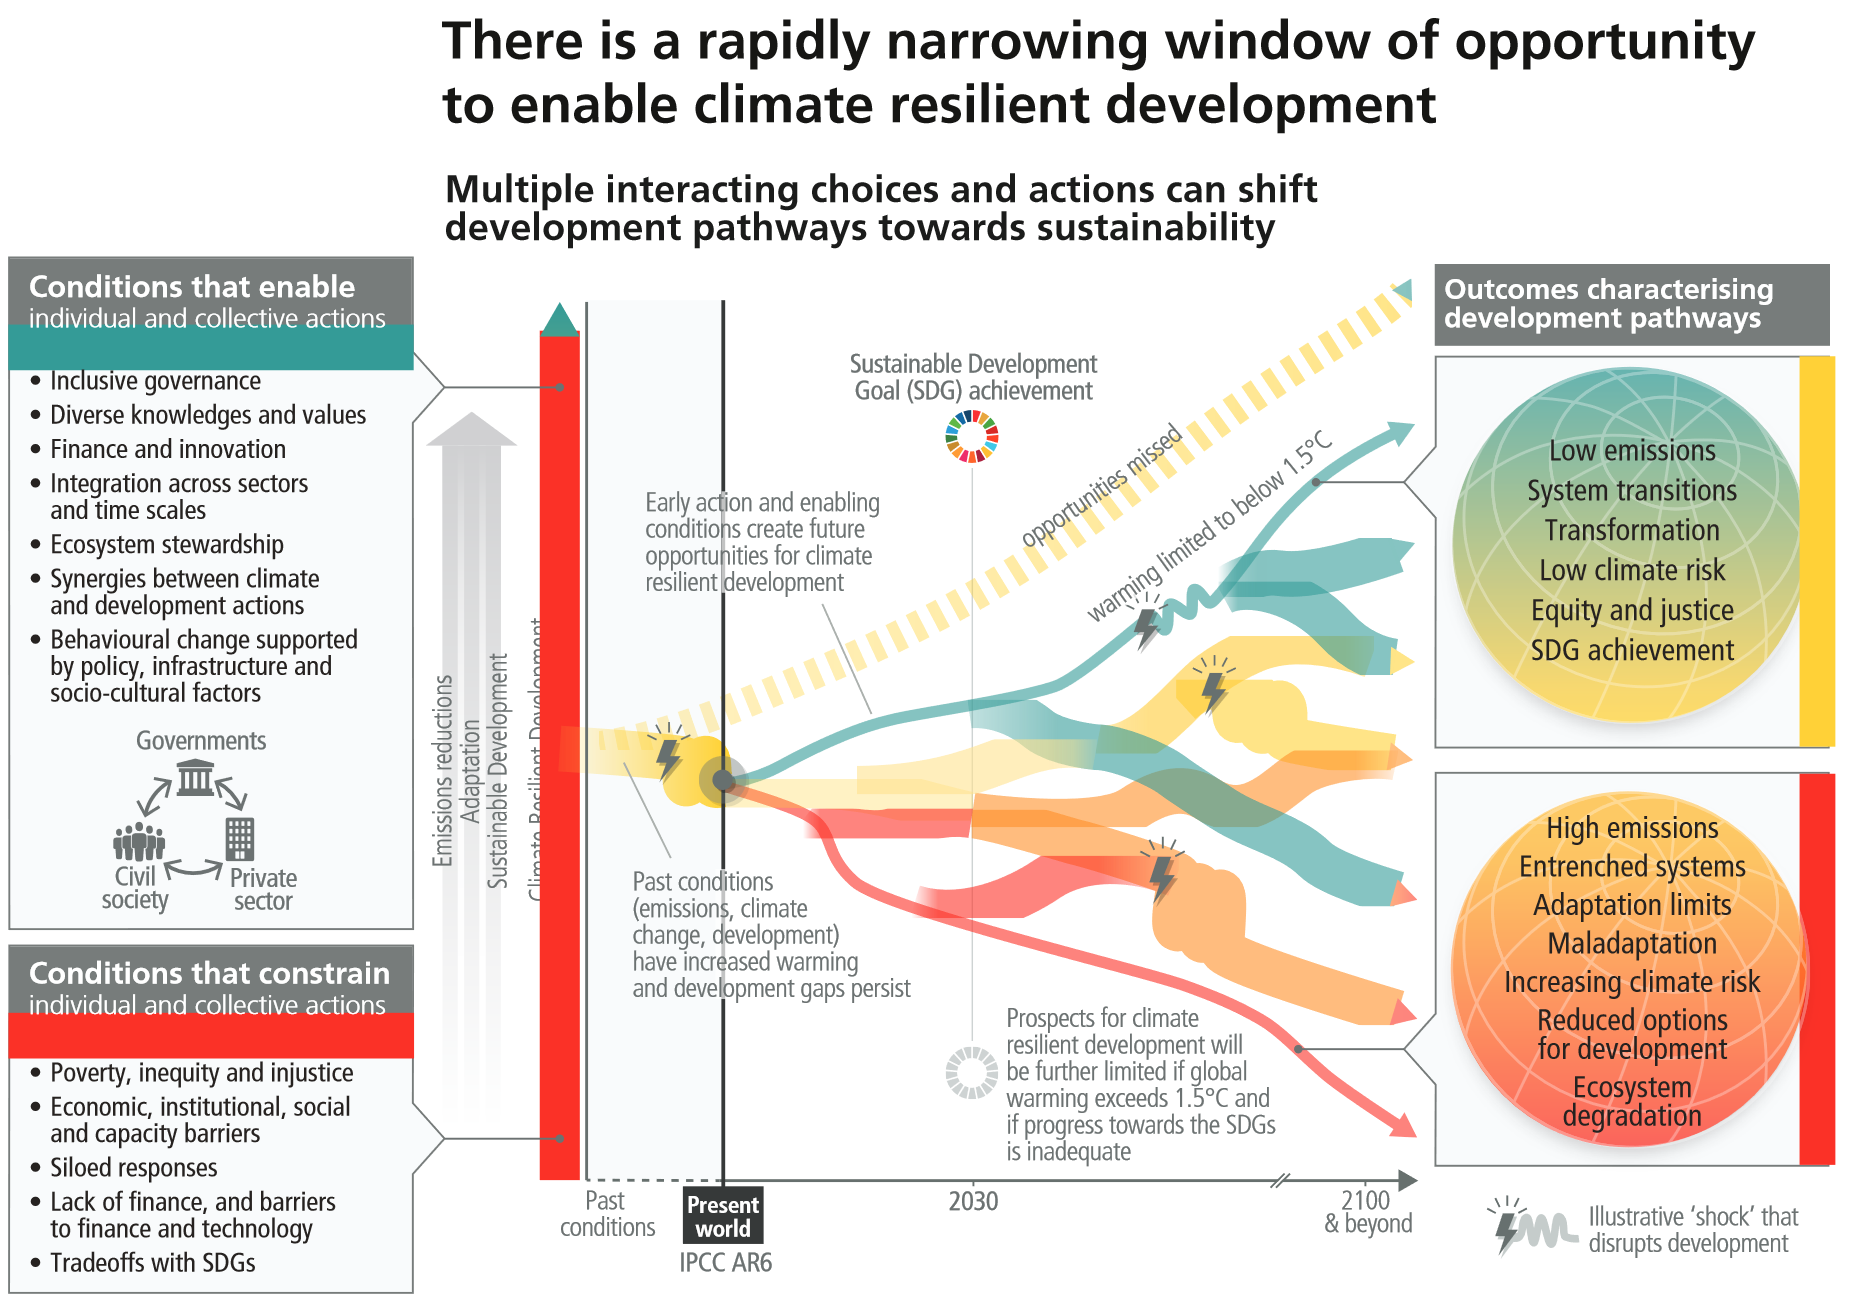
\includegraphics[width=\linewidth]{figures/trajectoire_spm6.png}
    \legende{Les trajectoires possibles pour atteindre les objectifs de développement durable}{Chaque fléche représente symboliquement un chemin de développement possible. Plus les flèches sont rouges, et plus le développement est loin des Objectifs de développement Durable et vulnérable aux aléas climatiques. Cette figure, issue du rapport de synthèse du GIEC (SPM.6) \textcite{lee_ipcc_2023}, montre que les décisions prises aujourd'hui influe les trajectoires possible demain. Elle illustre comment les concepts de trajectoires et de scénarios sont centraux dans le choix du chemin de développement.}
    \label{fig:pathways}
\end{figure}

Si l'existence de celui-ci ainsi que l'ampleur des conséquences qu'il induit ne font plus de doute, les actions à mettre en œuvre et les choix à faire pour le limiter et s'en protéger sont moins consensuelles. Elles font l'objet de nombreux débats, aux niveaux nationaux mais aussi internationaux dans la diplomatie climatique. Un des défis de ces décisions est l'incertitude qui les entoure : on ne connait pas les conséquences de chaque décision, et pourtant, il faut choisir un chemin. Une discipline cherche à éclairer cette route sombre, à la manière des phares d'une voiture : la prospective. Un outil particulièrement utilisé pour réduire cette incertitude est la modélisation, et particulièrement la modélisation intégrée. \\

%% Définition des termes

Pour aborder ce sujet, nous allons mobiliser plusieurs concepts, que nous serons amenés à redéfinir au fil de nos réflexions. 

% Modélisation 

D'abord, celui de \gls{modelisation}. Il s'agit d'une simplification de la réalité, qui permet de mieux la comprendre. Nous nous intéresserons particulièrement aux \gls{iam}, \textit{représentations simplifiées de systèmes sociaux et physiques complexes, qui se concentrent sur les interactions entre l'économie, la société et l'environnement}. Plus simple que les modèles climatiques, ils représentent à la fois des composantes physiques, économiques et énergétiques. Ils permettent ainsi de considérer simultanément ces sous-systèmes et leurs interactions. Les impacts du changement climatique représentent les effets délétères du changement climatique sur les sociétés ou les écosystèmes. 

% Responsabilité / choix / éthique / incertitude



%% Rappel du sujet

Nous nous intéressons donc ici à la modélisation des impacts du changement climatique, c'est-à-dire à la manière dont ils sont représentés dans les modèles intégrés. La question de recherche principale est : faut-il représenter les impacts du changement climatique dans les modèles ? Nous cherchons à y répondre par les sous-questions suivantes : Avec quel niveau de complexité faut-il représenter les interactions entre les sociétés et le climat ? Comment représenter les impacts-non monétaires ? Quelle est la responsabilité des modélisateur.ices sur l'interprétation qui est faite des modèles ?  \\

%% Plan 

\begin{figure}
    \centering
    
\includegraphics[width=\textwidth]{illustrations/intro.png}
    \legende{Les grandes étapes de la vie d'une modèle}{La modélisation consiste à représenter de manière simplifiée des phénomènes. Dans notre cas, il s'agit de phénomènes liés au changement climatique. Il existent avant toute forme de représentation (A), puis font l'objet d'une simplification (B). Ils sont ensuite interprétés (C), avant de conduire à des actions, telles que des décisions politiques (D). Chacune de ces étapes correspond à un chapitre : d'abord, on commence par évoquer les différents phénomènes qui sont modélisés (\ref{chapter:introduction}), puis on cherche à savoir comment ceux-ci sont représentés (\ref{chapter:litrev}). On analyse ensuite l'importance du choix de représentation sur les interprétations possibles (\ref{chapter:modelisation}), avant de discuter des enjeux éthiques liés à l'interprétation des résultats des modèles (\ref{chapter:ethique}). Enfin, on s'intéresse à la manière dont cette chaîne de production de connaissance alimente le débat public (\ref{chapter:socio}).}
    \label{fig:enter-label}
\end{figure}



Le  chapitre \ref{chapter:introduction} est consacré à une présentation du contexte scientifique et politique dans lequel s'inscrivent les \gls{damage function}. Il présente d'abord les différents risques climatiques, c'est-à-dire les raisons pour lesquelles on s'intéresse au changement climatique. Il poursuit en présentant l'intrication entre les sciences dures et la politique dans les négociations climatiques. Enfin, il présente les outils qui permettent d'éclairer ces décisions, notamment les modèles intégrés et leurs fonctions de dommage. Il sert avant tout à contextualiser l'environnement dans lequel se situe la modélisation intégrée. \\

Le chapitre \ref{chapter:litrev} présente une revue de littérature sur les \gls{damage function}. Il vise à présenter un état des lieux, qui se veut le plus complet mais non exhaustif, des fonctions de dommages qui sont utilisées (ou non) dans les modèles. Il est suivi d'une analyse de cet état des lieux, en classant les fonctions de dommages selon leur utilisation finale, leur forme ou encore les paramètres qui sont pris en compte. \\

Le chapitre \ref{chapter:modelisation} est la partie la plus expérimentale du mémoire. On cherche à quantifier l'effet des choix de modélisation sur le résultat des modèles, c'est-à-dire à quel point ils sont sensibles à leurs hypothèses. Dans un premier temps, on décrit la méthodologie pour pouvoir comparer les différentes fonctions entre elles, puis on réalise de nombreuses simulations avec de légères variations. Ces résultats font ensuite l'objet d'une analyse économétrique, pour quantifier l'effet des variations sur le niveau de dommage final et sa distribution. Cette expérimentation se fait dans le modèle \Gls{WILIAM}, auquel on a ajouté des fonctions reproduisant le comportement des fonctions de dommage d'autres modèles. \\

Dans le chapitre \ref{chapter:ethique}, on identifie des enjeux éthiques liés à la modélisation intégrée, que l'on tente d'éclairer à travers une approche épistémologique. Des exemples, tels que le choix de la forme, de la fonction, des paramètres ou encore des phénomènes représentés, sont analysés grâce à des philosophes des sciences. \\


Le chapitre \ref{chapter:socio} s'interroge sur la perception de ces enjeux éthiques chez les personnes qui participent au débat public sur les questions climatiques. À travers des entretiens semi-directifs chez une dizaine d'acteurs (scientifiques, techniciens, politiques et société civile), on cherche à établir quelle compréhension des enjeux éthiques transparait dans leur transposition au débat public. 

\begin{tcolorbox}[title=Avertissement]
    L'ensemble du code source utilisé dans le cadre de ce mémoire est accessible en libre accès sur \href{https://github.com/ggenelot/damage-functions-modeling}{ce dépôt github}. Par ailleurs, un des fils conducteurs de ce mémoire est de mener une réflexion épistémologique au plus près du modèle, et notamment du code. Cela est notamment rendu possible par \href{https://damage-functions-modeling.readthedocs.io/en/latest/index.html}{ce blog}, qui permet d'intégrer des morceaux de code. Tout au long du mémoire, des passages feront référence à des morceaux de code et/ou à des analyses qui y sont présentées. Il suffit alors de cliquer sur le lien (voir figure \ref{fig:logo}) pour y avoir accès. Il est également possible de se rendre sur le site en scannant le QR code (voir figure \ref{fig:qrcode}). \\

    \begin{center}
        \begin{minipage}{0.3\textwidth} % Ajustez la largeur selon vos besoins
            \centering
            
\includegraphics[width=3cm]{figures/logos/development.png}
            \captionof{figure}{Logo cliquable permettant d'accéder au site compagnon}
            \label{fig:logo}
        \end{minipage}%
        \hspace{0.05\textwidth} % Espace entre les deux images
        \begin{minipage}{0.3\textwidth} % Ajustez la largeur du minipage
            \centering
            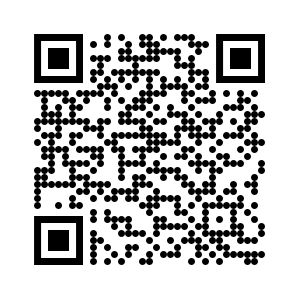
\includegraphics[width=3cm]{illustrations/frame.png} % Ajustez la taille du QR code selon vos besoins
            \captionof{figure}{QR code vers le site compagnon}
            \label{fig:qrcode}
        \end{minipage}
    \end{center}



    
\end{tcolorbox}

\begin{tcolorbox}[title=License]
    Toute la production originale est distribué sous la licence CC0. Ceci ne comprend pas les images et figures issues d'autres sources, qui appartiennent à leurs auteurs respectifs. De la même manière, le code source de WILIAM appartient à ses développeurs, et la propriété intellectuelle de chaque fonction de dommage revient à ses créateurs. \\

     \begin{center}
        \begin{minipage}{0.3\textwidth} % Ajustez la largeur selon vos besoins
            \centering
            
\includegraphics[width=6cm]{illustrations/ccby.png}
            \captionof{figure}{Distribué sous licence CC-BY}
            \label{fig:ccby2}
        \end{minipage}%
    \end{center}

\end{tcolorbox}


Les annexes proposent des documents complémentaires, notamment un index / glossaire, qui permet de mieux situés les termes les uns par rapport aux autres. 



\chapter{Impacts, risques et mesures}
\label{chapter:introduction}

\chapterabstract{Le changement climatique est à la fois extremement incertain, et nécessite des actions et des prises de décisions rapides et de grande envergure. Ce paradoxe a donné naissance à des institutions, comme le CCNUCC ou le GIEC, et à des outils, comme la modélisation intégrés. A chaque fois, l'objectif est de réduire l'incertitude et de favoriser le rapprochement entre l'action politique et la connaissance scientifique. Dans cette introduction, nous introduisons quelques uns des concepts cadres qui nous serons utiles tout au long du mémoire}

\newpage

%% Accroche
%Agir dans l'incertain : voici un des défis auquel nous soumet le changement climatique. L'action est nécessaire, tant l'ampleur de ces impacts est importante. Et l'incertitude est omniprésente : 

Les impacts du changement climatique sont de plus en plus présents dans le débat public : sécheresse, inondations, tempêtes font régulièrement les couvertures des journaux, et la plupart des partis politiques français ont pris position sur un programme climatique. C'est là une des spécificités du changement climatique : l'articulation très fine entre une réalité scientifique de plus en plus consensuelle d'une part, et de choix politiques incertains et normatifs d'autre part. 

%% Définition des termes

C'est justement la définition classique d'un risque : l'interaction entre un aléa et un enjeu. L'aléa, dans ce contexte, désigne un événement physique dont l'occurrence est possible : une canicule, un ouragan, la montée du niveau de la mer, etc. Un des effets du changement climatique est d'augmenter l'amplitude et la fréquence des aléas. L'enjeu est lié à ce que l'on a à perdre, c'est-à-dire ce qui a de la valeur et qui peut être affecté par la réalisation de l'aléa. 

%% Rappel du sujet
Nous nous intéressons au rôle des fonctions de dommage dans la formation de ces décisions politiques. 



%% Problématique
Nous tenterons ici de donner des éléments de contexte à la question suivante : 
Comment les fonctions de dommage des modèles intégrés permettent-elles de prendre en compte les risques climatiques ? Celle-ci s'accompagne d'autres questions : Quels sont les risques climatiques ? Comment sont pris en compte ces risques dans la gouvernance mondiale et nationale ? Et quels outils permettent d'éclairer ces prises de décision ? 



%% Annonce du plan 
Ce chapitre est construit en trois parties. Dans une première partie, nous nous intéresserons aux impacts du changement climatique, en les classant en trois types : les effets de tendance, qui sont linéaires ; les effets ponctuels et catastrophiques ; et les effets de seuil, ou tipping points. Nous aborderons dans une deuxième partie la manière dont les institutions internationales se sont organisées pour faire face à ces risques, et comment ces questions articulent des composantes scientifiques et politiques. Enfin, dans une troisième partie, nous détaillerons certains des outils qui ont été développés pour répondre à ces enjeux : les modèles intégrés, leurs fonctions de dommage et le coût social du carbone. 




    \section{Le changement climatique : tendances et impacts}

Cette section décrit les impacts du changement climatique et la manière de les prendre en compte

\subsection{Les effets moyens}

% Presenter les rapports du GIEC

\subsection{Les catastrophes}

\subsection{Les tipping points}

Les points de bascule, ou tipping points, sont des évolutions d'un système où celui-ci se comporte différemment. 

\paragraph{Les risk tipping points}

Au-delà de la définition classique du tipping point, l'Université des Nations Unies propose, dans son rapport sur les risques interconnectés, une nouvelle définition des risques interconnectés. Un \textit{risk tipping point}, ou point de bascule des risques, désigne \textit{l'instant où un système socioécologique ne peut plus absorber le risque et réaliser ses fonctions}. Après le passage de ce point de bascule, la possibilité d'un impact catastrophique augmente substantiellement. Six risques sont identifiés comme particulièrement représentatif des effets systémiques d'un driver sur tous les autres : l'accélération de l'extinction de la biodiversité, la réduction de l'eau de surface disponible, la fonte des glaciers, les débris spatiaux, la chaleur trop importante, et un futur qui n'est plus assurable. Parmi ces points de bascule, quatre sont  reliés à l'augmentation de la température atmosphérique ou océanique, et quatre à l'augmentation de la concentration en gaz à effet de serre dans l'atmosphère. \cite{united_nations_university_-_institute_for_environment_and_human_security_unu-ehs_interconnected_2023}

Ce concept est intéressant pour deux raisons : d'abord, il illustre la complexité des systèmes physiques et sociaux, et la complexité de leur interaction. Ensuite, il montre que la prise en compte d'un impact par le moyen d'un seul mécanisme risque de sous-estimer cet impact, car cela ne permet pas de prendre en compte les réactions en chaines et les interactions entre les différents impacts. 

\section{Prendre des décisions dans l'incertain : le rapprochement de la science et du pouvoir}

\subsection{Historique des négociations climatiques}

\subsection{Le cadre général : CCNUCC et COP}

\subsection{La synthèse des connaissances actuelles : le GIEC}

\subsection{Loss and damages : dommages, responsabilité et évaluation}

\section{Les outils : de la modélisation intégrée}

\subsection{Les modèles intégrés, ou comment cartographier les dynamiques du monde}

\subsection{Le coût social du carbone}

\subsection{Les fonctions de dommage}

\begin{figure}
    \centering
    \begin{tikzpicture}[scale=1]

\def\figureheight{20} % Choisis la hauteur désirée
\def\nodedistance{\textwidth*1/3}
\def\verticaldistance{2cm}
\def\nodewidth{3cm}

% Trajectory
\draw[line width = 2pt, rounded corners=8pt] (0,0) -- node[midway, below]{Les premières intuitions} (\textwidth,0) -- (\textwidth,-\figureheight*1/3) -- node[midway, below]{L'essor de la climatologie}(0,-\figureheight*1/3) -- (0,-\figureheight*2/3) -- node[midway, below]{Naissance du \textit{régime climatique}}(\textwidth,-\figureheight*2/3);


% Phase 1 : les premières intuitions


\node (1822) at (0,0.5) {1822};
\node (fourrier) [rectangle, draw, above of = 1822, text width=\nodewidth, text centered, yshift=2cm]{
Fourrier théorise l'effet de serre \\
\includegraphics[width=\linewidth]{images/Fourier2.jpg}
};

\node (1859) [right of = 1822, node distance = \nodedistance] {1859};
\node (tyndall) [rectangle, draw, above of=1859, text width=\nodewidth, text centered]{John Tyndall};

\node (1896) [right of = 1859, node distance = \nodedistance] {1896};
\node (farrhenius) [rectangle, draw, above of=1896, text width=\nodewidth, text centered]{Svante Arrhenius};

\node (1938) [right of = 1896, node distance = \nodedistance] {1938};
\node (callendar) [rectangle, draw, above of=1938, text width=\nodewidth, text centered]{Guy Callendar};

% 1822 : Joseph Fourrier
% 1859 : John Tyndall
% 1896 : Svante Arrhenius
% 1938 : Guy Callendar


% Phase 2 : l'essor de la climatologie

% Phase 3 : l'essor du régime climatique


% Information boxes
\draw[fill=blue!20] (0.5,-1) rectangle (2.5,-2);
\node at (1.5,-1.5) {Création du GIEC};
\draw[fill=green!20] (7.5,-1) rectangle (9.5,-2);
\node at (8.5,-1.5) {Première COP};
% Add more information boxes as needed
\end{tikzpicture}
    \caption{Caption}
    \label{fig:enter-label}
\end{figure}




\chapter{La relative diversité de la représentation des dommages}
\label{chapter:litrev}
\newrefsegment

\PEEL{Les manières de représenter les dommages du changement climatique varient selon leur niveau de désaggrégation, le type de modèle utilisé (simulation / optimisation), leur calibration et les phénomènes qu'elles prennent en compte. }{Nordhaus et Stern se disputent sur la valeur du taux d'actualisation (avec pourtant les mêmes modèles). Le SCC est calculé aux US alors que les dommages ne sont pas pris en compte dans les modèles de l'IIASA database. Il y a une forte utilisation des indicateurs économiques. }{Ces différents duels montrent la diversité de choix possibles offerts aux modélisateur.ices.}{Répondre à ces questions est un choix important, qui dépasse le pure cadre technique pour rejoindre la dimension éthique.}


\chapterabstract{Les fonctions de dommage permettent de modéliser les impacts du changement climatique sur d'autres parties du modèle. Elles peuvent varient par leur existence, forme, calibration ou par les paramètres ou secteurs qu'elles prennent en compte. Pourtant, un changement dans ces fonctions peut radicalement faire changer le fonctionnement d'un modèle, et ainsi les résultats et les conclusions qu'on en tire. Cette partie s'intéresse donc aux différentes fonctions de dommage qui existent dans la littérature.}

%%Accroche
Les modèles intégrés sont ainsi derrière de nombreuses publications qui informent le débat public : rapports du GIEC, Stern Review, revue du coût social du carbone. Ils ont donc un rôle de premier plan dans la prise de décisions sur les questions climatiques, sur les options qu'ils estiment possibles ainsi que sur les conséquences anticipées de telle ou telle action. Un élément clé de cette modélisation est la prise en compte des impacts climatiques. 


%%Définition des termes

%%Rappel du sujet
Les différentes formes de fonction de dommage dans les modèles intégrés

%%Problématique
Quelles sont les fonctions de dommages utilisées dans les modèles intégrés ? Et, plus précisement, quels modèles utilisent des fonctions de dommage ? Quels phénomènes sont représentés ? Quelles variables entrent en compte, et comment sont-elles paramétrisées ? 

%% Annonce du plan
Dans une première partie, nous détaillerons la méthodologie utilisée pour obtenir la base de donnée des fonctions de dommage. Dans une seconde partie, nous la décrirons avec différentes statistiques descriptives. Enfin, nous aborderons trois points critiques des fonctions de dommage : leur forme; leurs paramètres; et la calibration. 

\begin{methodbox}[Revue de la littérature]
Pour obtenir une base de données des différentes fonctions de dommage, nous avons cherché à fusionner plusieurs sources de données. D'abord, l'IAM Consortium publie sur son site internet les documentations de nombreux modèles intégrés, sous la forme d'un wiki. Ces fiches sont rédigées par les équipes des modèles - ce qui permet d'avoir une source primaire sur les informations concernant les modèles - mais sont souvent incomplètes. En revanches, des "cartes", qui détaillent les principales caractéristiques de chaque modèle, sont également disponibles. Ce sont principalement celles-ci qui sont utilisées dans la base de données. Une autre source de données est le fichier des scénarios utilisés par le GIEC. Celui-ci permet d'avoir des informations sur chacun des scénarios soumis pour l'AR6, et d'avoir accès à de nombreuses informations : modèle utilisé, vetted ou non, impacts climatiques pris en compte ou non. A ces différentes sources, on ajoute manuellement des modèles, basée sur une lecture aléatoire de la littérature. Ils comprennenent notablement les modèles utilisés par l'agence interagence du coût social du carbone, ceux cités par Souffron et Jacques, ceux utilisés par les SSP, ainsi que d'autres modèles intégrés trouvés par littérature interposée. 
Le monde de la modélisation est très vaste, les modèles souvent compliqués à comprendre et parfois peu transparents. Ainsi, il a toujours été préféré de se baser sur des sources explicites. Bien qu'un véritable effort pour chercher à avoir une vision sur le plus de modèles possibles, cette étude ne peut pas être considérée comme un recensement exhaustif des modèles intégrés ni de leurs fonctions de dommage. \\ \gls{latex}

Une fois cette première liste de modèles obtenue, un premier tri est effectué entre ceux qui intègrent une fonction de dommage et ceux qui n'en intégrent pas. On considére ici les fonctions de dommages explicitement définies telles quelles, bien que d'autres fonctions puissent in fine avoir un comportement similaire. Ainsi, pour certaines, on a une connaissance explicite : par exemple, les fiches de l'IAMC comportent une case sur les impacts modélisés. Pour les autres, on considère qu'elles n'ont pas de fonction de dommage si les termes "damage function" ou "damage" ne sont pas présents dans leur documentation ou les publications associées, et s'il n'est pas fait mention de fonctions de dommage dans d'autres sources. \\

Pour chaque modèle incluant des fonctions de dommage, on cherche dans sa documentation la description de ces fonctions de dommage. La plupart du temps, celle-ci comporte une équation et les variables associées. Un script Chat-GPT est alors utilisé sur la partie du document qui est décrit la fonction de dommage. Celui-ci interprète et met en forme (sous la forme d'un tableau CSV) toutes les variables présentes dans cette fonction. Elles sont alors contrôlées visuellement. Cette étape est repétée pour chaque fonction de dommage. Une fois les variables de chaque fonction de dommage d'un modèle identifiées, ce fichier est téléversé dans la base de données, à l'aide du logiciel Airtable, dans la table 'Variable'. \\

Une fois les variables insérées dans leur table, les fonctions de dommage sont incluses dans la table 'Damage functions'. Chaque fonction est assortie à un nom, soit celui-donné dans la publication, soit choisi selon le contexte. Sont également ajoutés le nom du modèle, le numéro de l'équation, l'annotation zotero et le DOI de la publication, afin de pouvoir retrouver rapidement la fonction de dommage. Sont alors ajoutés d'une part les variables qui viennent en entrées de l'équation, et la variable qui sur laquelle l'équation agit. \\

Enfin, une autre table est ajoutée : celle des risques identifiés par le GIEC. Ceux-ci sont issus du rapport de synthèse de l'AR6, et la classification est faite par l'auteur. Lorsqu'une fonction de dommage décrit un des risques identifiés par le GIEC, elle se voit liée à celui-ci. 



\end{methodbox}

\begin{figure}
    \centering
    %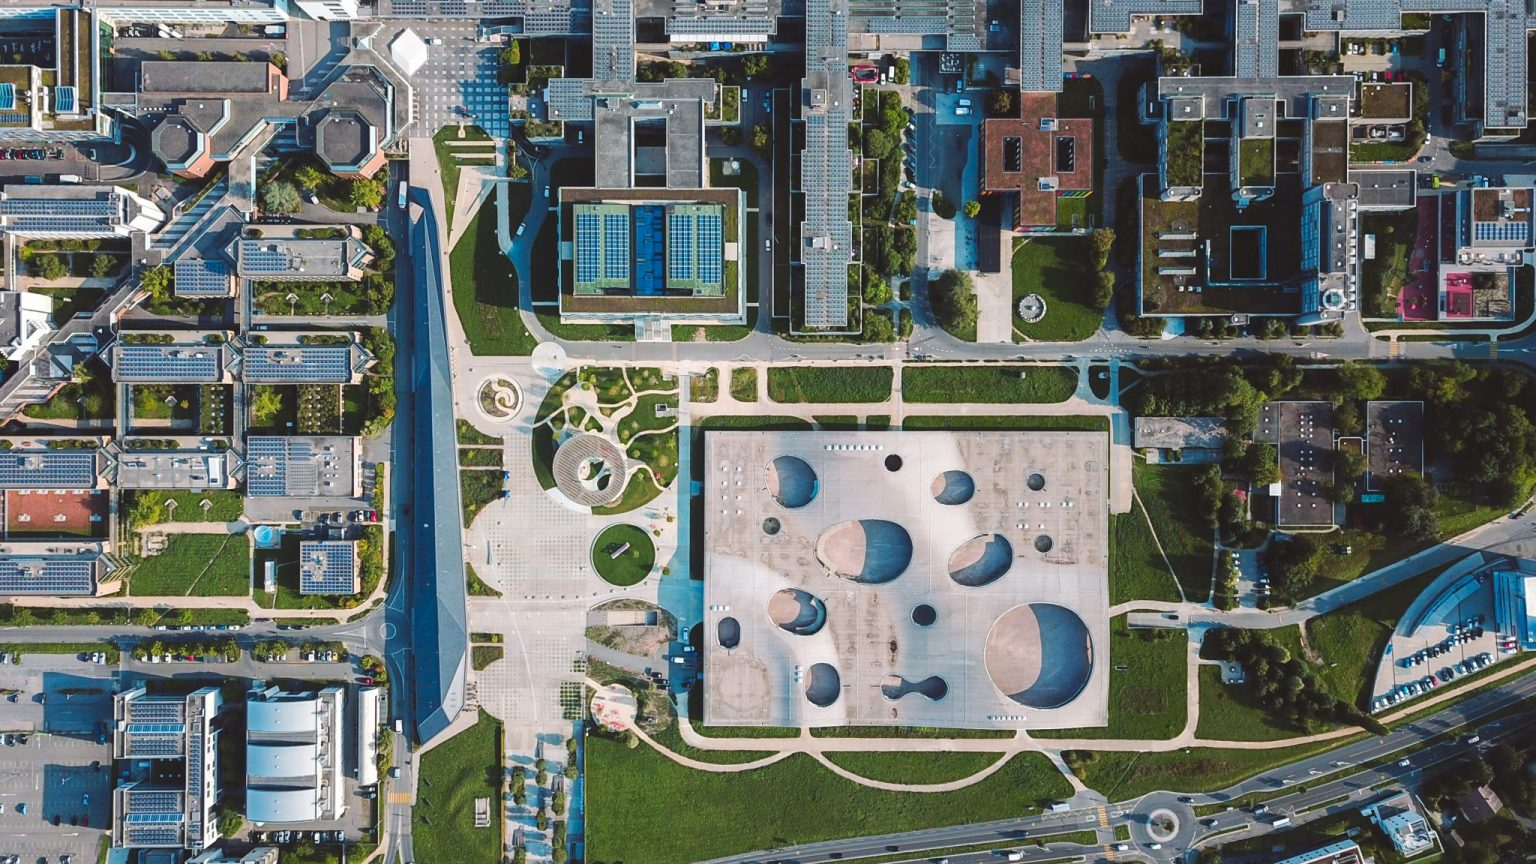
\includegraphics{figures/campus.jpg}
    \legende{Processus de sélection des modèles.}{Les modèles sont sélectionnées selon plusieurs critères : présence dans une des bases de données (GIEC, SCC, SSP, IAMC) ou dans une review. Ils sont ensuite comparés selon leurs caractéristiques.}
    \label{fig:méthodo-litrev}
\end{figure}

\section{Tour d'horizon des modèles et de leurs fonctions de dommage}

Les modèles intégrés sont très variés. Ils ont des histoires différentes (issus de l'énergie, de l'économie ou du climat), des perspectives différentes (en particulier entre les États-Unis ou l'Union européenne), des questions différentes, des choix de modélisation différents (simulation ou optimisation). 

Revue de la littérature se classe en 3 catégories : la construction des IAMs, la comparaison des résultats des IAMs, les articles iam par iam

\subsection{Une littérature composée d'article par modèle ou de méta-analyses}

La littérature existante s'articule autour de trois axes. D'abord, il y a une abondante littérature autour des modèles. En effet, chaque modèle fait l'objet de nombreuses publications pour en présenter la structure, puis pour en donner les résultats. Il y a par ailleurs de nombreuses ressources appartenant à la littérature grise : des blogs, du code source, des rapports aux commanditaires, des modèles, etc. Ensuite, il y a des méta-analyses qui comparent les résultats des modèles; enfin, tout un pan de la littérature s'intéresse à la structure même des modèles, à travers des comparaisons entre modèles. 

\subsubsection{Documentation et résultats de chaque modèle}

\paragraph{Les modèles sont accompagnés d'analyses}

La principale source d'information que l'on a sur les modèles est les publications scientifiques qui en présentent les résultats.
Il s'agit de publications qui démontrent quelque chose ou répondent à une question (voir, par exemple, \cite{int_panis_externe_2000, dafermos_how_2021, baumstark_remind21_2021, dafermos_stock-flow-fund_2017, cherp_global_2016, burke_global_2015}). Le modèle et/ou la fonction de dommage y sont peu décrits (au plus une équation sans paramétrisation), souvent dans la section méthodologie. Ces articles sont intéressants car ils permettent de comprendre la finalité des modèles, les conditions pour lesquelles ils ont été conçus. En revanche, ils ne permettent pas à eux seuls de reproduire l'analyse ou de la modifier. 


\paragraph{Le niveau de documentation et d'ouverture varie considérablement}

Une autre source de documentation est la littérature grise qui accompagne les publications scientifiques. On en trouve des formes très variées, telles que des rapports (voir \cite{medeas_guiding_2019, asbjorn_aaheim_grace_2018, european_commission_ginfors-e_2022, european_commission_gem-e3_2013, nordhaus_dice_2013}), des \emph{working papers} (voir par exemple \cite{dafermos_stock-flow-fund_2017, giraud_coping_2016, calvin_gcam_2019, bosetti_witch_2006, ghersi_imaclim-p_2014}), des blogs (voir par exemple \cite{tol}

\paragraph{}

\subsubsection{Sur les résultats des IAMs}





Meta analyse des estimations du niveau du changement climatique
\cite{howard_few_2017} => 

\cite{gillingham_modeling_2018} gillingham => peut être à mettre dans la partie \ref{chapter:modelisation} ?

\cite{keppo_exploring_2021} => grosse revue de littérature sur les IAMs

\cite{harmsen_integrated_2021} => évaluation des IAMs à travers une méthodologie précise




\subsubsection{Sur la structure des IAMs }

\paragraph{Il existe des fonctions de dommage, mais sous des modèles semblables entre eux et orthodoxes.}

Dans une importante revue de littérature sur l'évaluation des dommages climatiques par les modèles intégrés, \cite{diaz_quantifying_2017} passe en revue les caractéristiques et contraintes liées aux fonctions de dommages. Elle inspecte en particulier DICE, FUND et PAGE, qui sont trois modèles conçus spécifiquement pour évaluer monétairement les impacts. Elle formule de nombreuses critiques : l'extrapolation à de hautes températures ou à d'autres régions, le choix des impacts représentés, l'absence d'interaction inter-régionales ou temporelles, l'absence de représentation de l'adaptation, des données scientifiques datées, la représentation lacunaire de l'incertitude, et d'autres encore. 

Cet article a servi de réference à la suite de ce travail. Néanmoins, les modèles représentés sont similaires, avec des objectifs similaires et produits par des communautés scientifiques proches. Or, la plupart des critiques faites par Diaz sont liées à des méthodes de modélisation ou  à des hypothèses générales. Pour comparer ces modèles et défier ces hypothèses, il faut sortir de cette communauté.  \\


Nous nous intéressons donc à d'autres revues de littératures, plus large, mais permettant d'avoir un plus large panel de modèles. 

\paragraph{Chercher des modèles plus divers permet de répondre à certaines des critiques}


Par exemple, \cite{souffron_successful_2024} cherchent à explorer la diversité des modèles, et montrent qu'un plus large panel de modèles permet de mieux guider les politiques publiques. Ils montrent que les modèles orthodoxes sont particulièrement limités. Ils présentent ensuite des modèles alternatifs, mettant en avant les atouts et contraintes de chacun. Enfin, ils émettent des recommandations de caractéristiques que pourraient avoir des modèles idéaux, notamment le fait d'avoir des fonctions de dommage. 






\cite{souffron_successful_2024} => présente plein de modèles et les commente. Pas vraiment une revue de littérature sur les damage functions mais plus général, permet de bien se repérer dans la littérature + grosse emphase sur les modèles hétérodoxes

\cite{review of information on models}  Une revue des différents modèles 

\paragraph{D'autres revues comparent des hypothèses plus varéies dans les modèles}

\cite{krey_looking_2019} => comparaison des hypohtèses technologiques des modèles

Sur les types de modèles : 
\cite{mercure_modelling_2019} => présente les principales différences entre les modèles de simulation et d'optimisation, et montre que c'est aussi une différence paradigmatique. 

\paragraph{La place particulière de l'IAMC}


Il y a une multitude de ressources liées à la modélisation des dommages dans les modèles intégrés. Il n'existe pourtant pas de plateforme unique permettant de recenser toutes les formes de fonctions de dommage, leurs effets, atouts et contraintes. 

\section{Méthode : construction de la base de données}

\begin{table}[]
    \centering
    \begin{tabular}{c|c}
         &  \\
         & 
    \end{tabular}
    \legende{Les différents modèles recensés et leurs fonctions de dommage}{Description rapide}
    \label{tab:my_label}
\end{table}

\subsection{Premiers indicateurs quantitatifs}

\begin{figure}
    \centering
    %\includegraphics[width=0.5\linewidth]{}
    \legende{Visualisation graphique des différents modèles}{Description rapide}
    \label{fig:enter-label}
\end{figure}

\subsection{Les principaux modèles}

On présente ici rapidement des modèles, leurs caractéristiques générales et la forme de leur fonction de dommage. Il s'agit surtout de montrer la diversité des approches de modélisation, et non d'avoir un recensement systématique. Les lecteurs plus curieux trouveront plus de caractéristiques en suivant le lien. \blog{https://damage-functions-modeling.readthedocs.io/en/latest/1_introduction/functions.html}

\subsubsection{DICE}

DICE veut dire XXX et constitue une des premières tentatives de modéliser les relations entre l'économie et le climat. Il comporte une fonction de dommage, extremement simplifiée. 

\begin{equation}
\begin{array}{ll}
    & \displaystyle  \Delta = \psi_{1}T_{AT}(t) + \psi_{2}[T_{AT}(t)]^{2} \\
    & = [0.0]T_{AT}(t) + [0.003467][T_{AT}(t)]^{2}
\end{array}
\label{eq:df_dice2023}
\end{equation}

\subsubsection{FUND} 

A l'inverse, FUND présente un niveau de désagrégation assez avancé. Il y a de nombreuses fonctions de dommage, qui sont utilisées les unes dans les autres. Leur forme générale est d'obtenir un niveau de dommage à partir d'une élasticité entre un phénomène et un autre. \\

Par exemple, l'impact du changement climatique sur l'agriculture est construit par la somme de trois canaux : d'une part, l'impact du niveau de changement climatique; d'autre part, la vitesse de ce changement (représenté en \ref{eq:fund_A2}); enfin, l'augmentation de la fertilisation des plantes. 

\begin{equation}
    A_{t,r}^{r}=\alpha_{r}\left(\frac{\Delta T_{t}}{0.04}\right)^{\beta}+\left(1-\frac{1}{\rho}\right)A_{t-1,r}^{r}
    \label{eq:fund_A2}
\end{equation}

D'autres impacts sont aussi représentés, tels que l'impact du niveau des eaux sur le littoral, les écosystèmes, les domages liés aux cyclones tropicaux et extra-tropicaux, etc. , et ce par différents biais : des dommages directs (monétaires), et la monétarisation de perte de vie ou de perte de temps de vie. 

\begin{equation}
    D_{t,r}^{\nu}=D_{1990,r}^{\nu}Q_{r}^{\nu}\left(T_{t}-T_{1990}\right)^{\beta}\left(\frac{y_{t,r}}{y_{1990,r}}\right)^{\gamma}
    \label{eq:fund_HV}
\end{equation}

\begin{equation}
    V S L_{t,r}=\alpha\left(\frac{y_{t,r}}{y_{0}}\right)^{\gamma}
    \label{eq:VSL}
\end{equation}

\subsubsection{Autres formes quadratiques}

Les formes quadratiques issues de DICE/RICE ont été grandement critiquées (voir section \ref{ss:forme}), et d'autres formes quadratiques sont apparues. C'est le cas notamment dans DEFINE (\ref{eq:DEFINE}), dont on peut trouver une forme très similaire dans le Giraud Stock-Flow consistent model. Il s'agit d'équations qui, comme DICE, sont extrememnt simplifiées et aggrégée, mais la forme de la relation est différente. 

\begin{equation}
    \Delta T = 1 - \frac{1}{1 + \eta_1 TAT + \eta_2 TAT^2 + \eta_3 TAT}
    \label{eq:DEFINE}
\end{equation}

\subsubsection{Autres formes non quadratiques}



\section{Trois questions centrales}


\subsection{La forme : comment représenter un phénomène qui n'existe pas encore ?}
\label{ss:forme}

La première difficulté quant à la représentation des impacts du changement climatique est le choix de la forme de la fonction de dommage. En effet, les phénomènes à l'origine des dommages climatiques sont à la fois incertains et récents. D'abord, les phénomènes physiques, dont on a du mal à avoir une représentation fiable et précise (voir notamment la section \ref{fig:tipping-point} sur les tipping points). Ensuite, et peut être plus encore, l'interaction entre ces évenements et les sociétés humaines est extremement difficile à comprendre, et donc à modéliser. Exercice de simplification, la modélisation nécessite pourtant d'extraire des lois générales de phénomènes particuliers, pour pouvoir établir des relations entre eux. \\

Ainsi, il est déjà très difficile de choisir une forme fonctionnelle qui soit adaptée. On peut contrer cet argument en avançant que la pratique de la modélisation doit assumer cette simplification. De ce point de vue, un modèle ne vise pas à reproduire la réalité ou des mécanismes réels, mais seulement à fournir un cadre explicatif suffisant pour rendre intelligible des choses qui ne l'étaient pas avant. \\

Le caractère récent des impacts du changement climatique, et encore plus de la prise en compte de ces effets en tant qu'effets du changement climatique, complique encore un peu la tâche. En effet, les séries temporelles étant courtes, il est difficile d'en extraire des formes fonctionnelles qui correspondraient effectivement à la relation entre les différentes variables. \\

Enfin, ces sources de données ne couvrent qu'un intervalle d'anomalie de température assez faible. En effet, on estime le réchauffement climatique actuel à environ 1.2 \textdegree C par rapport à la période pré-industrielle. Cependant, les estimations vont plus haut : l'accord de Paris pour le climat vise à avoir une réchauffement limité à 2 \textdegree C , et le plus proche possible de 1.5 \textdegree C; des estimations vont plus loin encore. Ainsi, des fonctions calibrées sur l'intervalle $[+0; +1.2]$ pourraient ne pas du tout capter les phénomènes observés dans le futur, sur un intervalle plus grand. Là réside un des grands défis de la modélisation des dommages : il s'agit de modéliser des phénomènes qui n'existent pas encore, et qui surviendront dans un contexte probablement très différent sur de nombreux aspects de celui dans lequel a lieu la modélisation. 

\begin{figure}[ht]
\centering

\includegraphics[width=\textwidth]{results/shape.png}
\legende{Niveau de dommage en fonction de l'augmentation de température}{Différentes formes fonctionnelles peuvent avoir un pouvoir explicatif important sur l'intervalle $[+0; +1.2]$, sur lequel on dispose de données empiriques, tout en divergeant grandement pour des valeurs plus haute de changement de température. Une fonction de dommage correctement calibrée pour des phénomènes observés n'est pas forcément calibrée pour les phénomènes futurs.}
\end{figure}


Le choix de la forme de la fonction (ou des formes des fonctions lorsqu'il y en a plusieurs) est donc très incertain. S'aider de données empiriques ne résout qu'une partie du problème. Il est probable que ces relations changent grandement dans des conditions différentes, et il est dès lors impossible d'extrapoler les données actuelles. 

\subsection{Les paramètres : quel niveau de complexité faut-il, et que prendre en compte ?}

Une seconde difficulté réside dans le choix des paramètres à représenter. 

La figure \ref{fig:sankey} représente les liens que font les fonctions de dommages entre leurs paramètres et leurs résultats. Elle est tirée du tableau des fonctions de dommage, dont la construction est détaillée plus haut. Ce tableau contient toutes les fonctions de dommages recensées, ainsi que les paramétres entrants (inputs) et sortant (outputs) de la fonction de dommage. Par exemple, l'input de l'équation \ref{eq:DEFINE} est la température, et l'output est le niveau de dommage en proportion du PIB. La figure représente chaque relation $ \text{input} \mapsto \text{output} $. Il est possible qu'une fonction relie plusieurs inputs à un output, auquel cas elle est représentée par plusieurs traits. L'épaisseur des traits est proportionnelle au nombre de relations.


\begin{figure}
    %\centering
    %\includegraphics{}
    %\legende{Analyse en composantes principales des modèles.}{Les modèles sont classés selon beaucoup de composantes, pour identifier des similitudes ou des patterns.}
    \label{fig:ACP}
\end{figure}


\begin{figure}
    \centering
    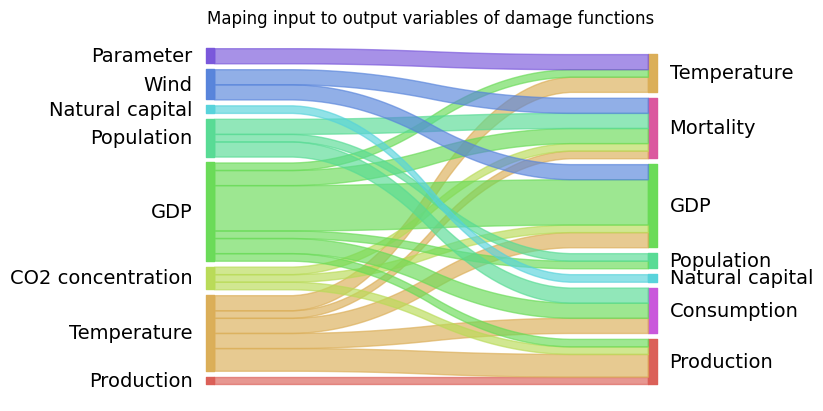
\includegraphics[width=0.9\linewidth]{figures/sankey.png}
    %\legende{Sankey diagram des différentes fonctions}{Les modèles ne prennent pas en compte tous les mêmes données en entrées, et elles ne permettent pas d'expliquer les mêmes phénomènes.}
    \label{fig:sankey}
\end{figure}

\subsection{La calibration : un \textit{"tiens"} vaut-il deux \textit{"tu l'auras"} ?}

\section{Trois querelles pour répondre à ces questions}

\subsection{Le taux d'actualisation : la querelle Nordhaus / Stern}

La controverse qui oppose William Nordhaus et Nicolas Stern est un exemple classique des enjeux éthiques et normatifs induit par la modélisation intégrée. Il est bien expliquée dans \cite{guigourez_10_2023}, sur lequel on va s'appuyer pour rappeler ici les enjeux de cette querelle. \\

William Nordhaus est un économiste des Etats-Unis. Au début des années 1990, il met au point le modèle DICE, qui est une des premiers à modéliser l'interaction climat - économie. Ce modèle sera ensuite mis à jour régulièrement, et sera suivi de RICE, un modèle plus régionalisé. Il obtient le Prix dit Nobel d'Economie en 2018 pour ses l'intégration du changement climatique dans l'analyse macro-économique que long terme\cite{yale}. Adepte de la théorie des choix publics, il pense que l'inaction climatique vient d'une mauvaise appréciation des coûts futurs du changement climatique, et qu'une analyse coût-bénéfice permet de suivre des trajectoires climatiques plus optimales. 
Sir Nicolas Stern a été vice-président senior de la Banque Mondiale de 2000 à 2003. Peu après, le gouvernement britannique lui commande un rapport sur les effets du changement climatique sur l'économie. \\

Les deux auteurs utilisent des modèles intégrés : Nordhaus utilise DICE, et Stern utilise PAGE. Les deux modèles sont similaires en termes d'hypothèses et de fonctionnement. Ces modèles sont des modèles d'optimisation, qui visent à donner un coût optimal à une tonne de carbone. Ils sont d'ailleurs utilisés pour calculer le coût social du carbone (voir figure \ref{fig:scc}). Pour pouvoir comparer le coût de politiques publiques aujourd'hui, aux gains ultérieurs (c'est-à-dire aux dommages futurs évités), il faut pouvoir comparer ces deux grandeurs. \\

Cependant, on considère que la valeur de l'argent dans le futur est plus faible qu'aujourd'hui. De nombreux facteurs permettent d'arriver à cette conclusion : le futur est incertain, et il est donc possible que ces événements ne se réalisent pas; ou alors que les générations futures soient capable de mieux y faire face; ou tout simplement, nous préférons nos générations aux générations ultérieures. C'est une formalisation de l'adage : \emph{un tiens vaut deux tu l'auras}. La question est donc de savoir \emph{à quel point} les dommages futurs sont moins importants que ceux d'aujourd'hui, ou encore combien de \emph{tu l'auras} un \emph{tiens} vaut-il ? \\

Formellement, on retient la structure suivante : 

\begin{equation}
    r_t = \delta + \eta g_t 
    \label{eq:disc_rate}
\end{equation}

où $r_t$ représente le taux d'actualisation de la consommation à l'instant $t$, $\delta$ représente la préférence pure pour le présent, $\eta$ l'élasticité marginale de l'utilité en fonction de la consommation, c'est-à-dire à quel point les agents peuvent adapter leurs préférences,  et $g_t$ le taux de croissance de la consommation. \\

Cette formulation permet d'intégrer la préférence pure pour le présent, appelée aussi taux d'actualisation de l'utilité, dans la fonction de consommation. C'est ainsi qu'elle est implémentée dans DICE et PAGE. À partir d'ici, nous nous intéresserons uniquement à $\delta$, que nous appellerons taux d'actualisation. \\

Nordhaus utilise comme paramètres $\delta = 1.5\%$ et $\eta=2$, tandis que Stern utilise $\delta=0.1\%$ et $\eta=1$. Ainsi, Stern considère que l'on doit prendre en compte les dommages causés aux générations futures (presque) comme s'ils survenaient maintenant; tandis que Nordhaus considère qu'il faut les prendre en compte en retirant 1,5\% de leur valeur chaque année. \\

À partir de ces simples hypothèses, et en utilisant des similaires, les auteurs obtiennent des résultats drastiquement différents. Stern suggère des investissements massifs et rapides, tandis que Nordhaus promeut de faibles investissements aujourd'hui, pour n'investir que plus tard. 

\cite{guigourez_10_2023} => description de la querelle

\begin{figure}
    \centering
    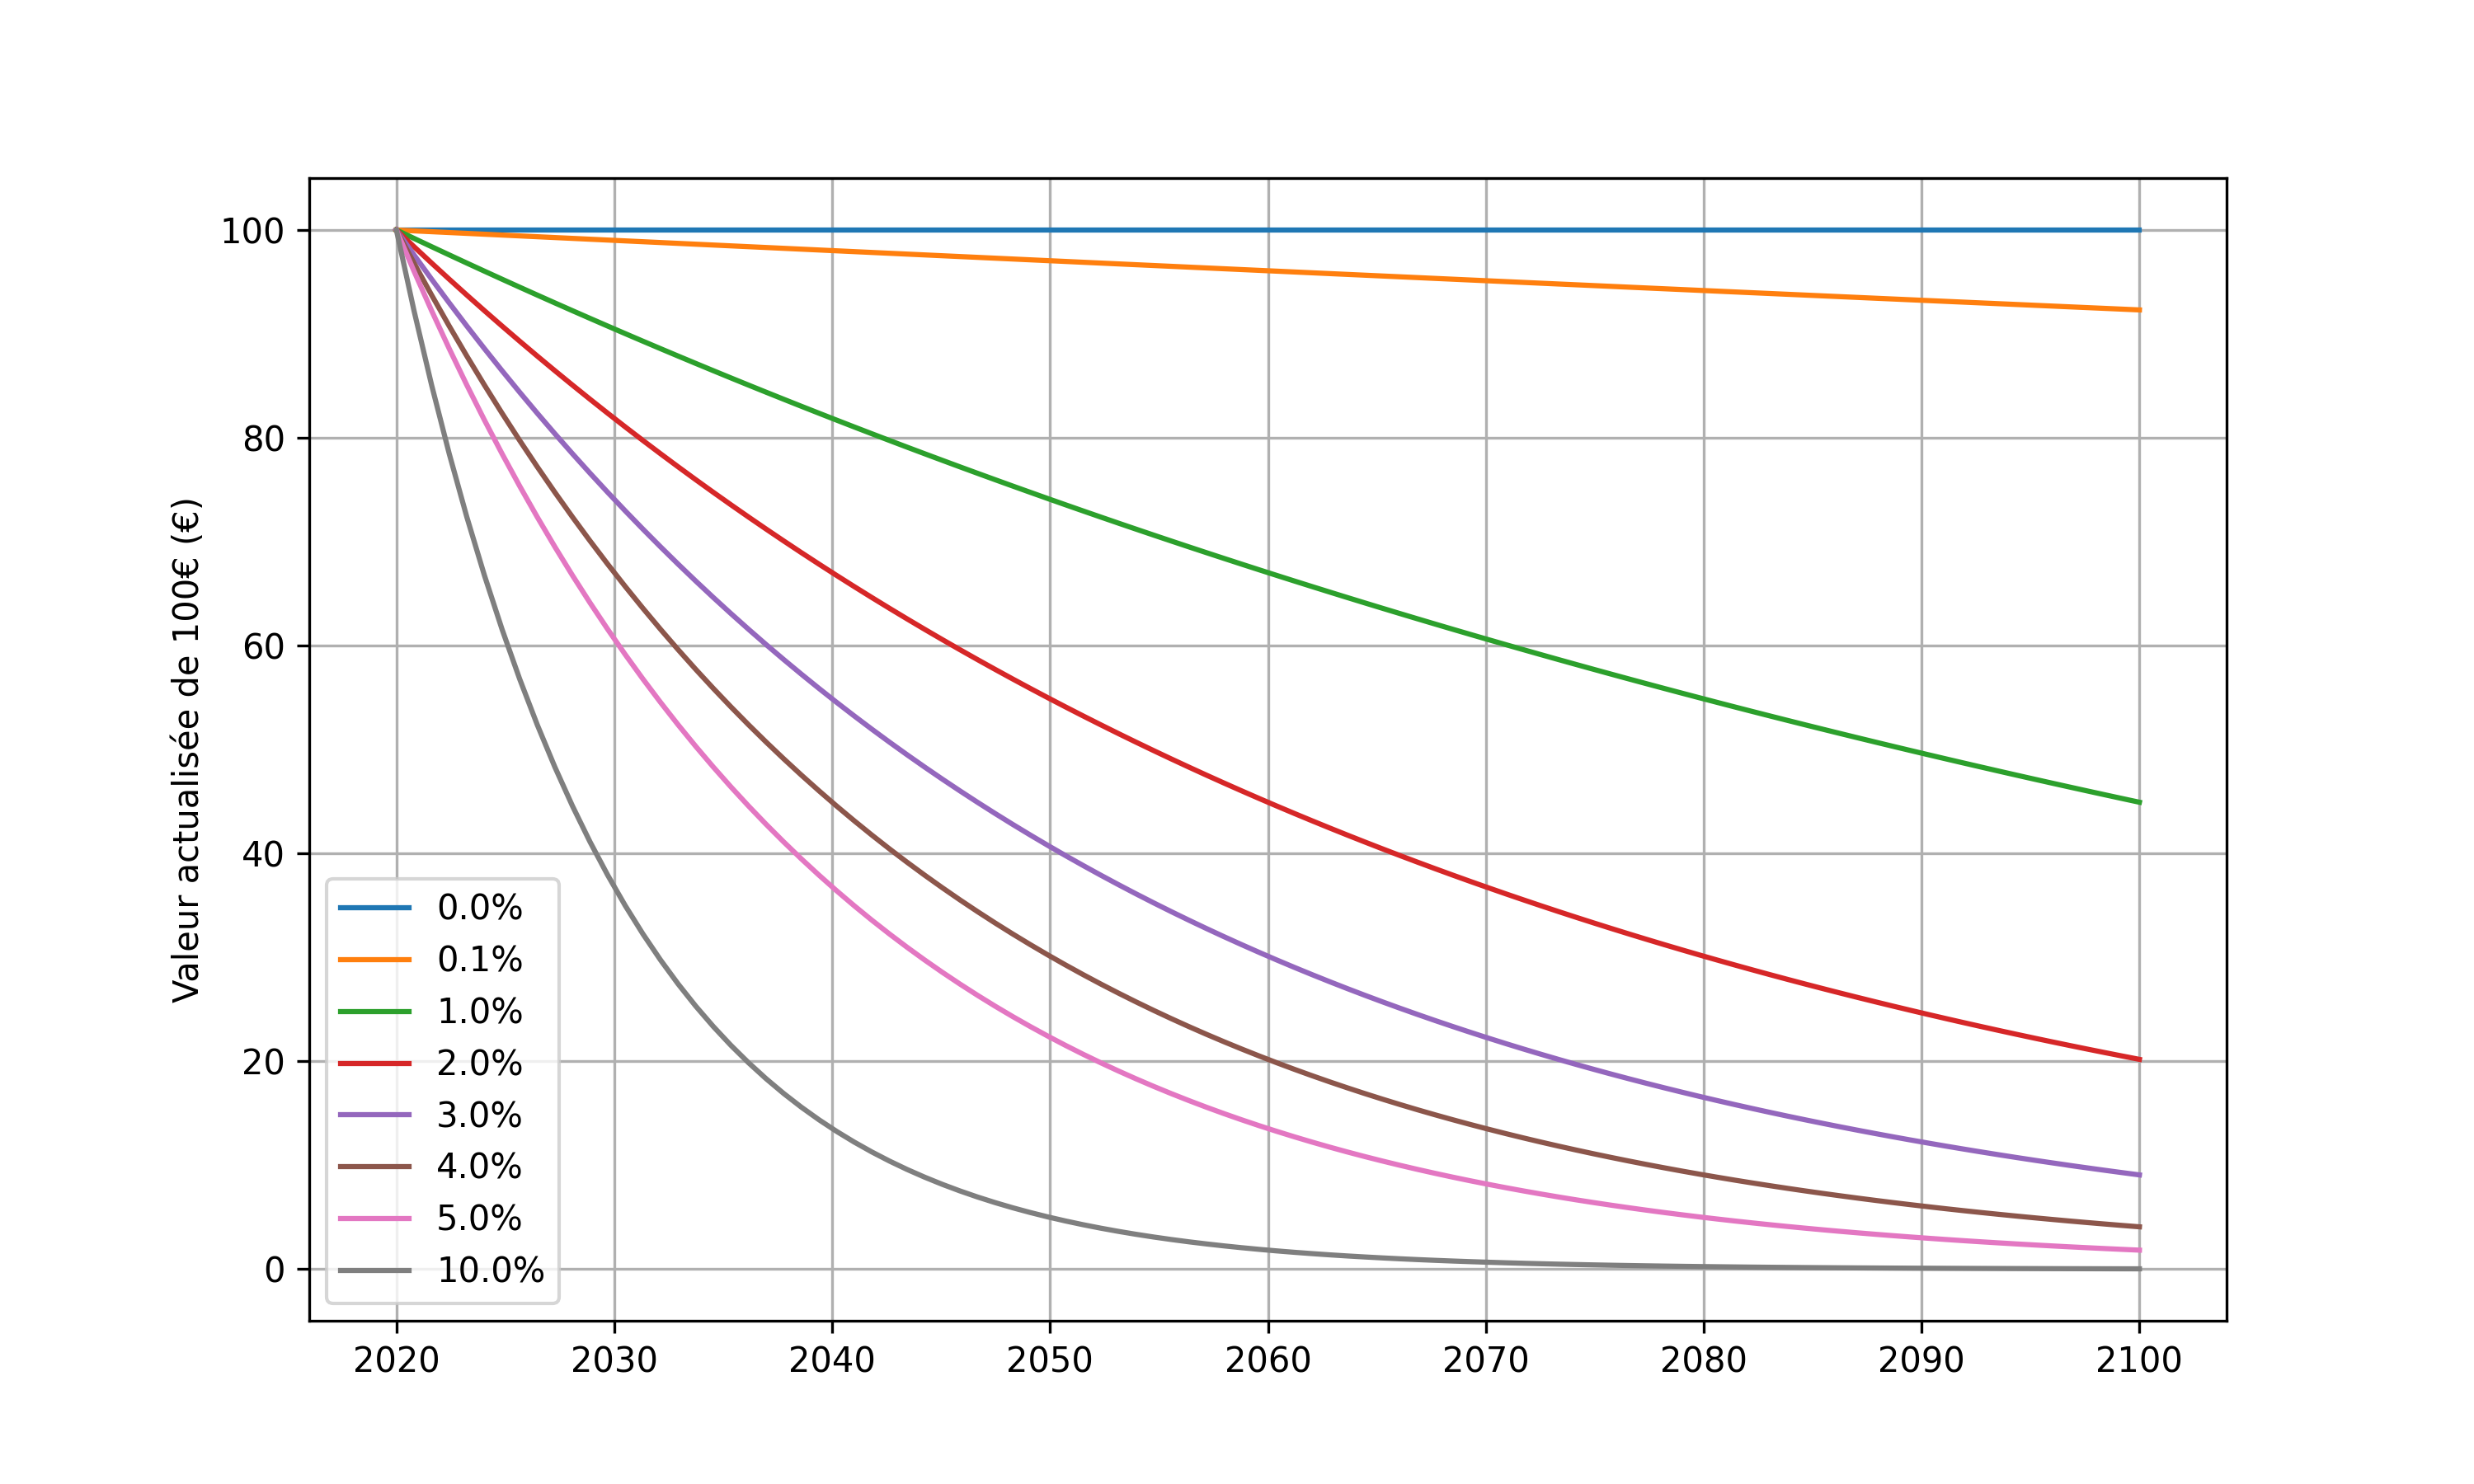
\includegraphics[width=\linewidth]{results/actualisation.png}
    \legende{Valeur actualisée selon le temps et le taux d'actualisation}{Graphique qui représente la valeur d'une unité monétaire dans le temps, actualisée au présent, selon le taux d'actualisation. En jaune, celui choisi par Nordhaus, et en bleu celui choisi par Stern. Clé de lecture : avec un taux d'actualisation de 3\%, 100\$ de dommage en 2080 ne valent que 18\$ en 2020, alors que 100\$ de 2040 valent 56\$. }
    \label{fig:discount-rate}
\end{figure}

\subsection{Pourquoi représenter les dommages ? Les SCC vs le reste du monde}

Comme nous avons pu le voir, les critiques quant à la quantification et la monétarisation des dommages sont déjà nombreuses. Se pose donc la question suivante : faut-il représenter les dommages, et si oui, pourquoi et comment ? Pour éclairer ce dilemne, nous allons nous pencher sur deux une distinction particulière, entre les modèles qui représentent les dommages et ceux qui ne le font pas. \\

D'une part, certains modèles représentent des dommages de manière explicite. Ce sont essentiellement des modèles utilisés pour mesurer le coût social du carbone. Les arguments qui sont avancés par leurs défenseurs sont solides. Nous vivons dans un monde où la valorisation économique est centrale. Conformément à la théorie économique, et notamment à celle consacrée aux biens communs et aux externalités, si on ne peut pas compter la valeur de quelque chose, et surtout qu'elle ne s'impose pas à nous lors des transactions, alors cette valeur est invisible. De ce point de vue, et malgré les nombreuses limites (souvent assumées d'ailleurs) de la modélisation de ces phénomènes, il est nécessaire de représenter les dommages dans le modèle, même de manière imparfaite. En effet, selon ce point de vue, ne pas les représenter revient à les négliger, les omettre, ou en d'autre terme, à leur attribuer arbitrairement une valeur nulle. 
C'est dans cette perspective que se place de nombreux modèles, qui cherchent à proposer de nouvelles manières de représenter les dommages. Nombreux sont ceux qui, en réponse à la simplicité de la représentation de Nordhaus, ont proposé des fonctions de dommage toujours plus complexe, prenant en compte plus de mécanismes. 
\\

D'autre part, on peut argumenter que la représentation de ces dommages donne une fausse sensation de certitude. D'une part, elle done l'impression que le modèle est plus réaliste, en ce sens que ce qu'il dit \textit{serait} plus proche de la réalité et moins sujet aux travers de la simplification car justement plus complexe. Pourtant, on peut argumenter que la représentation des dommages, y compris quand elle est sophistiquée, fait appel à de nombreuses hypothèses, notamment concernant la permanence des phénomènes qui ont lieu. On a alors un modèle qui non seulement n'est pas forcément plus fiable ou plus proche de la réalité, mais qui est en plus nettement moins lisible, compréhensible - et dont les limites ne peuvent que très difficilement être interprétées et critiquées. 

\subsection{Compter ce qui n'a pas de prix : la difficile monétarisation}



\begin{figure}
    \centering
    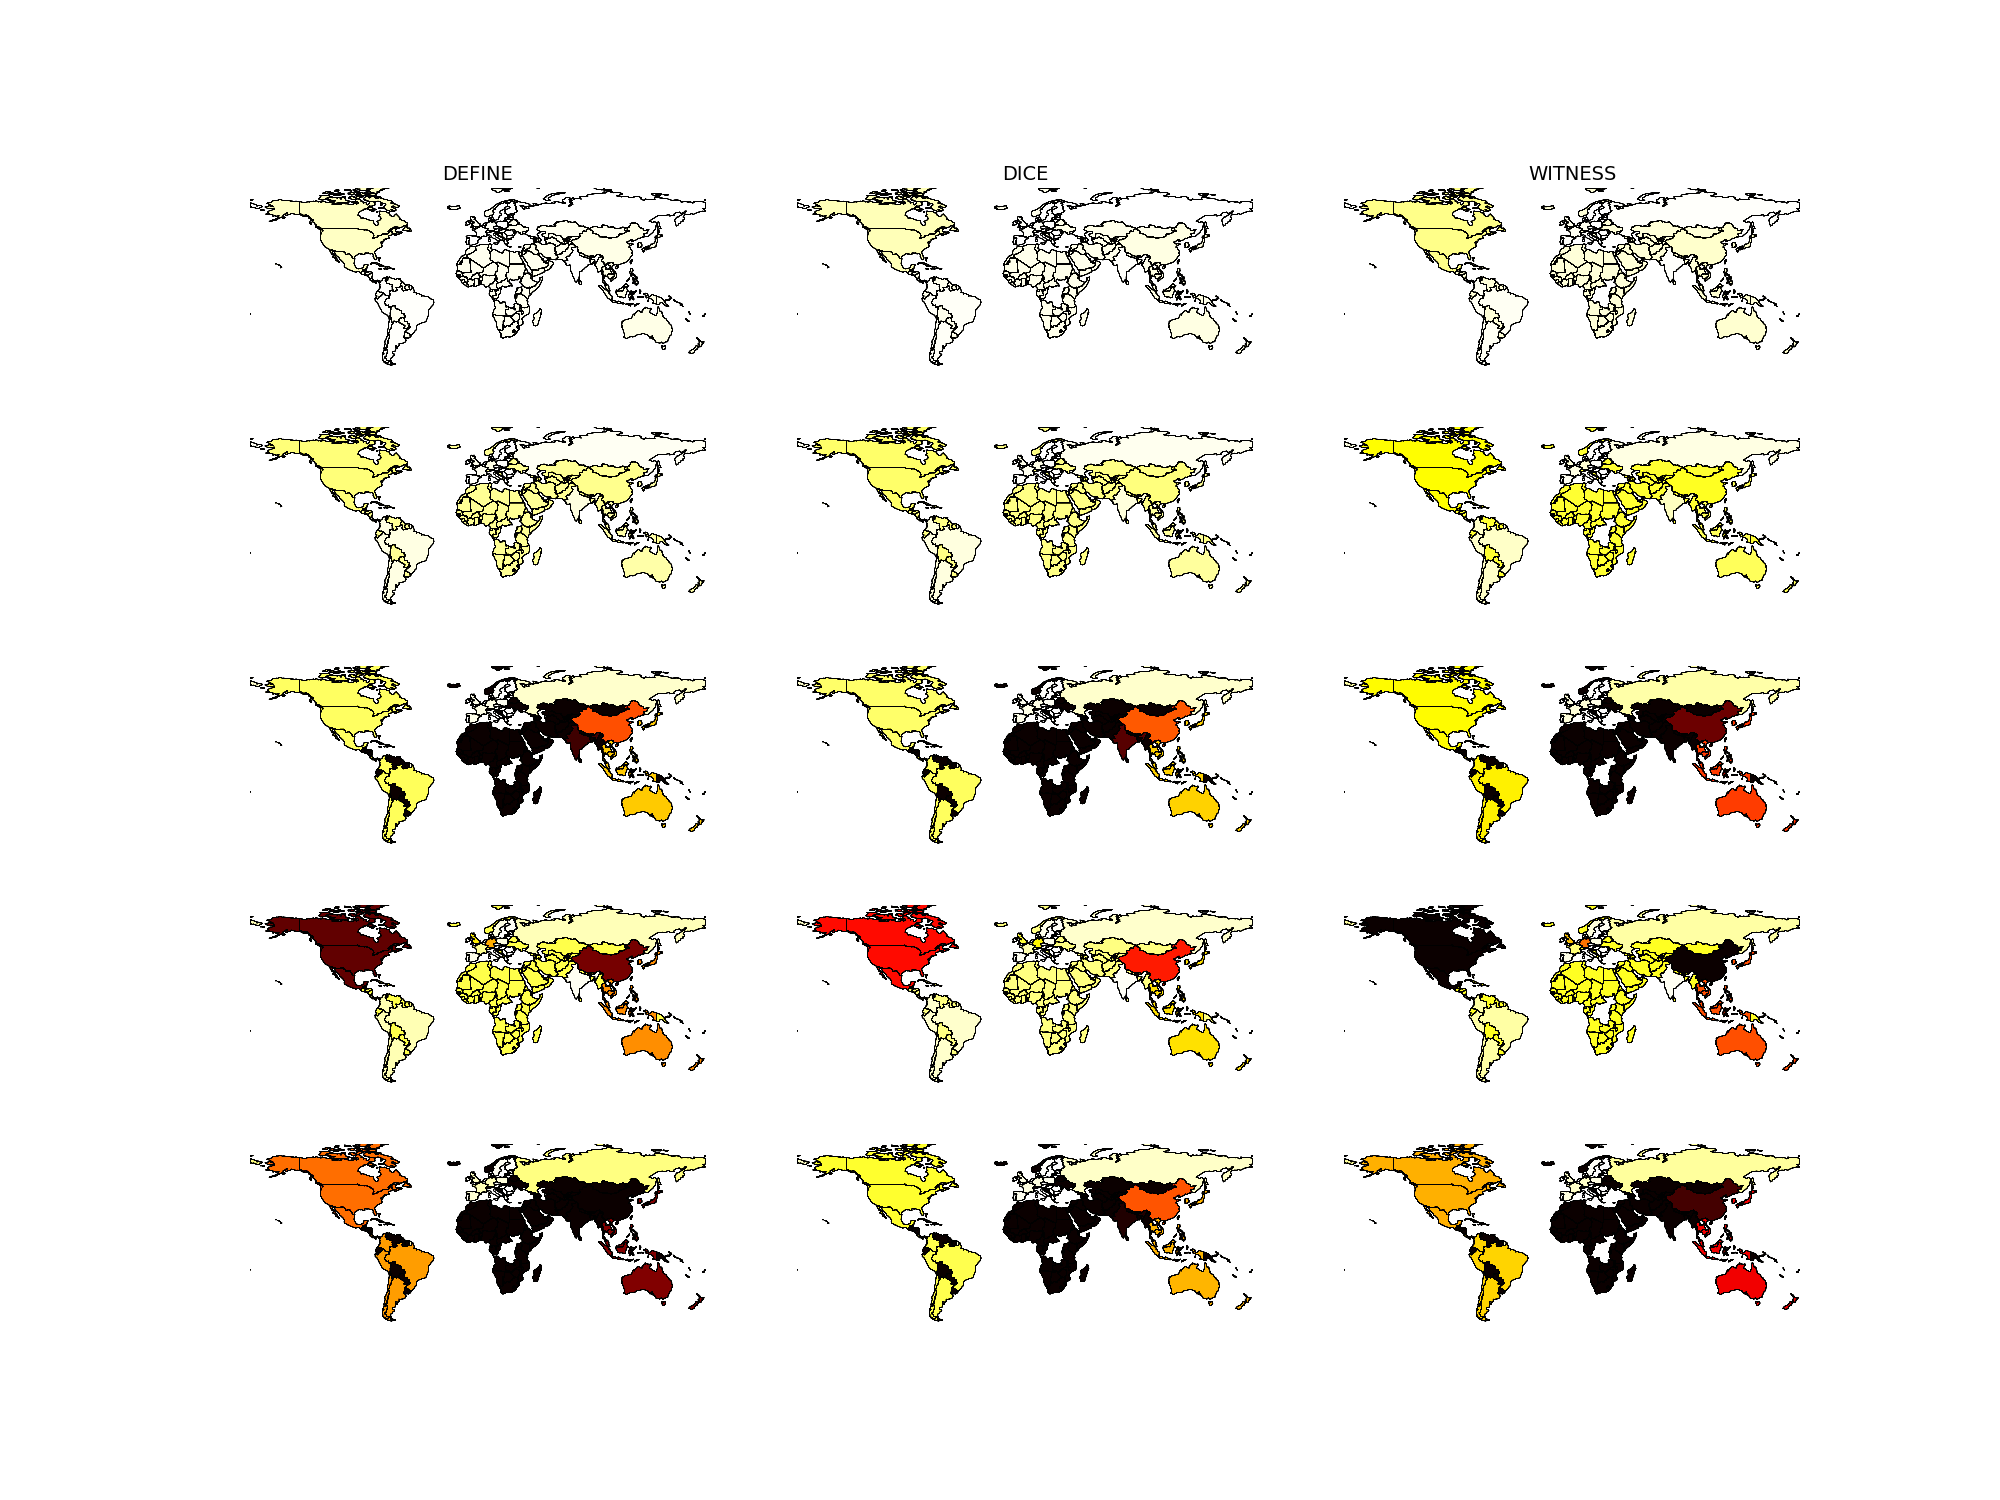
\includegraphics[width=\linewidth]{results/carte_progressive.png}
    \legende{Double progression du niveau de dommage}{Le niveau de dommage suit une double progression. D'une part, il augmente avec le temps (qui est lui même très lié au niveau de réchauffement); d'autre part, il augmente avec le modèle : certains modèles donnent des niveaux de dommage plus importants que d'autres.}
    \label{fig:carte-progressive}
\end{figure}



\chapter{Rendre visible : quantifier les choix éthiques}
\label{chapter:modelisation}
\newrefsegment
\PEEL{Les différents choix de modélisation abordés plus haut ont une variation sur le niveau de dommage importantes, presque aussi / plus importante que d'autres facteurs souvent pris en compte (incertitude, scénario climatique).}{On utilise une analyse économétrique pour essayer de quantifier ce phénomène. }{Même si les résultats ne sont pas super forts, on voit qu'il y a une variation importante qui est issue de la variation de ces paramètres éthiques.}{Le modèle ne donne pas de vérité absolue, il sort ce qu'on y a fait entrer => les modèles sont profondément politiques, et reflètent en ce sens une certaine conception du monde.}




\chapterabstract{Ce chapitre propose une approche plus économétrique des effets de la modélisation des fonctions de dommage. On utilise le modèle WILIAM, qui pourrait devenir un modèle de référence de la commission européenne, auquel on change les fonctions de dommage. On le fait tourner avec de nombreux scénarios, pour obtenir des résultats. On réalise ensuite une étude économétrique de ces résultats, pour savoir qu'elle paramètre a le plus d'effet sur les résultats du modèle.}

\cite{errickson_equity_2021} => il peut y avoir une plus grande variation du SCC selon l'équité que selon l'incertitude climatique

Nous avons vu dans le chapitre précédent que les modèles varient dans leurs choix de représentations des dommages. De plus, ces différents choix semblent tous valables à leur manière : les phénomènes représentés sont incertains, et cette variabilité représente surtout l'incertitude qui entoure ces phénomènes. Pourtant, ce sont bien les mêmes phénomènes; il ne devrait donc pas y avoir de différence entre les modèles. Ces différences sont donc apportées exclusivement par les choix de modélisation; or, elles peuvent être importantes, et donner des conclusions radicalement différentes, donnant lieu à des interprétations opposées. La querelle entre Nordhaus et Stern, évoquée plus haut, en est un exempe éloquent. 

Il est donc intéressant de voir dans quelle mesure ces variations influencent le comportement du modèle. En effet, si elles sont peu importantes comparées à d'autres facteurs, elles ne compromettent pas le message du modèle. En revanche, si elle joue un rôle central dans le fonctionnement de celui-ci, alors il convient de leur accorder une place majeure, tant dans l'analyse des résultats que dans la conception. 

On cherche donc à mesurer quantitativement les effets de ces variables sur les résultats du modèle pour répondre à la question suivante : les variations induites par les choix éthiques sont-elles du même ordre de grandeur que les variations issues de variables physiques ou de choix de modélisation ? 



On définit ici la notion de paramètre éthique : elle désigne les paramètres qui n'ont pas vocation à représenter un phénomène physique ou social observable, mais plutôt à représenter une valeur morale. Le taux d'actualisation, par exemple, entre tout à fait dans cette définition. En effet, il représente l'importance accordée à l'équité intergénérationnelle. bien qu'il y ait eu des tentatives d'observer empiriquement cette valeur, notamment en s'intéressant au taux de préférence pure pour le présent dans les prêts de long terme, il semble difficile de penser que cette valeur soit valable à plus long terme ou dans d'autres contextes. Plutot, il apparait que ce paramètre reflète un système normatif, et relève de ce fait plutôt du choix moral que du choix technique. Se pose alors la question suivante : quelle part de la variation du niveau total de dommage est-elle expliquée par ces paramètres éthiques.  On s'intéressera ici à une autre dimension éthique, qui est celle de l'équité spatiale. Pour ce faire, on construit un pondérateur géographique, qui pondère le niveau de dommage par région selon le niveau de revenu.

Dans cette partie, on développe un protocole expérimental qui vise à mesurer le niveau de dommage produit par différents modèles, différentes fonctions de dommages et des variations du pondérateur géographique. On régresse ensuite les données obtenues pour mesurer quantitativement la part de la variation qui est expliquée par ces différents paramètres. 

\section{Cadre conceptuel}

Le cadre conceptuel général de cette expérience est celui de la modélisation intégrée. Il s'inscrit en cela dans la lignée des réflexions développées dans le chapitre \ref{chapter:introduction}. Il semble néanmoins nécessaire de préciser quelques points. \\

\subsection{Choix du modèle}

D'abord, le choix du modèle. Pour réaliser cette expérience, nous avons choisi d'utiliser le modèle WILIAM, pour plusieurs raisons. 

\paragraph{Modèle Open-source}WILIAM est un modèle Open-Source, ce qui signifie que l'ensemble du code source est disponible en ligne, avec une licence permettant une utilisation, diffusion et modification du programme sans limites. C'est nécessaire puisqu'on a ainsi accès à tous le code source, ce qui permet de travailler sur une base solide; on peut également le modifier librement, ce qui est au coeur de l'expérience; enfin, on peut le diffuser librement aussi, ce qui est fait à travers le dépôt GitHub et le blog. Par ailleurs, bien que ce ne soit pas en soi une garantie de qualité, l'utilisation de l'open source permet d'améliorer la robustesse et la transparence des modèles, puisque chacun peut voir les hypothèses, proposer des modifications, et corriger des erreurs. 

\paragraph{Application aux politiques publiques} WILIAM est issu du projet LOCOMOTION, financé par la Commission Européenne. Il répond à une demande de celle-ci de s'équiper d'un nouveau modèle. Ainsi, WILIAM est un modèle qui vise à répondre à des questions de politique publique. 

\paragraph{Modèle complexe} WILIAM est un modèle particulièrement complexe : il compte près de 4000 variables. Cela le rend particulièrement vulnérable aux problématiques de transparence et de complexité excessive que nous développerons plus tard. Néanmoins, cela nous permet d'avoir un modèle le plus comple possible. Cela permet d'intégrer les fonctions de dommage facilement, car les variables sont déjà existantes. 

\paragraph{Modèle de simulation} WILIAM est un modèle de simulation. Cette caractéristique est importante car elle permet de voir les valeurs de chaque paramètre à tout moment, mais aussi de représenter des paramètres non monétaires. De plus, ça le rend moins sensible aux critiques de normativité inhérente aux modèles d'optimisation \ref{}. 

% \section{Présentation des données}


\section{Méthode}

\subsection{Données}

\subsubsection{Variables descriptives}


\begin{methodbox}[Modélisation des fonctions de dommage dans WILIAM]

Pour modéliser les fonctions de dommage dans WILIAM, on commence par créer un nouveau repo sur github, dans lequel on télécharge le code source de WILIAM. On s'assure que tout est fonctionnel, et que le modèle tourne bien. La visualisation du modèle se fait grâce au logiciel VENSIM. \\

On rassemble les sources de données disponibles des modèles : code source, documentation et / ou publications qui y font référence. Ces sources n'offrent pas le même niveau d'information. Par exemple, les modèles dont on ne trouve pas le code source mais uniquement des publications sont plus difficiles à modéliser car il manque souvent des informations cruciales, telles que les valeurs obtenues pour les paramètres. \\

Une fois la définition de la fonction identifiée, on les modélise à l'aide de l'interface graphique du logiciel VENSIM. On sauvegarde régulièrement en réalisant des \textit{commit} sur GitHub pour garder une trace de la progression.
    
\end{methodbox}

\begin{methodbox}[Conversion des paramètres selon les bonnes zones géographiques]

    Le modèle WILIAM comporte 35 régions. En revanche, les autres modèles n'ont pas nécessairement le même découpage géographique. Deux cas se distinguent : soit le modèle est agrégé au niveau mondial; on peut alors utiliser les fonctions de dommage région par région, sans besoin de les changer. Soit le modèle possède des régions, et il faut alors convertir les régions du modèle A en régions de WILIAM pour avoir la bonne paramètrisation. Ce deuxième cas de figure est particulièrement vrai dans le cas du modèle FUND, qui a des régions très différentes de celles de WILIAM, et qui repose beaucoup sur de la paramétrisation. Il faut donc convertir les paramètres des régions de FUND en régions de WILIAM. 

    Par ailleurs, il est à noter que si la documentation de FUND est très complète et accessible en ligne, les tables de paramètre ne sont pas disponible dans un format facilement lisible tel que CSV. La méthode retenue a été de lire la page de la documentation (en Markdown), et de la découper table par table puis valeur par valeur à l'aide d'un script python, qui permet ensuite d'enregistrer ces données dans un format lisible par VENSIM. Ces opérations sont longues et peuvent être source de nombreuses erreurs. Ainsi, le non-partage des données dans un format standard est un vrai frein à la reproductibilité. \\
    
    On utilise alors un script Python qui désagrège les zones de FUND en pays, et qui associe à chaque pays sa zone dans WILIAM. 
    
\end{methodbox}

La plupart des fonctions de dommage dépendent du niveau de revenu par habitant, de plusieurs manières. Le premier cas de figure est qu'elles donnent un niveau de dommage qui est exprimé en proportion du PIB. On a alors un niveau de dommage absolu qui est plus grand dans les régions plus riches, puisque le PIB est lui-même plus grand. Ce point est essentiel, en particulier dans les modèles d'optimisation. En effet, ces modèles cherchant à trouver la solution la moins couteuse, ils vont être beaucoup plus sensibles aux dommages dans les pays ayant un PIB plus important que dans les pays ayant un niveau de revenu plus faible. \emph{De facto}, ils vont chercher à minimiser les dommages dans les pays les plus riches, quitte à augmenter les dommages dans les pays les plus pauvres. \\

La deuxième manière est que la fonction de dommage intègre directement le niveau de revenu dans le calcul du niveau de dommage. Selon le signe de l'équation, cette méthode peut renforcer les effets dans les pays les plus pauvres, ou au contraire les augmenter. 

On peut finalement citer une technique permettant de monétiser des impacts non-monétaires, tels que des morts ou des années d'invalidité. La technique utilisée est assez classique en économie : il s'agit de calculer la valeur d'une vie statistique, ou \emph{value of a statistical life} (VSL). Cette méthode part de l'hypothèse que la valeur de la vie dans un lieu donnée correspond à un certain multiple du niveau de revenu par habitant dans ce lieu. On peut prendre en exemple la VSL du modèle FUND, qui prend la forme suivante : 

\begin{equation}
    VSL_{t, r} = \alpha (\frac{y_{t,r}}{y_0})^\epsilon
\end{equation}
où $t$ désigne l'année, $r$ désigne la région, $\alpha$ et $\epsilon$ des paramètres permettant de calibrer la fonction, $y_{t,r}$ le revenu par habitant dans la région $t$ à l'instant $r$, et $y_0$ un revenu de référence.  \\

Ce choix de modélisation pose de nombreuses questions. 
D'abord, d'un point de vue pragmatique. Les pays les plus pauvres sont susceptibles d'être les pays les plus impactés par le changement climatique, d'une part par une exposition plus grande à des phénomènes extremes, et d'autre part par une situation de pauvreté préexistante qui fragilise la résilience. 
Ensuite, pour des raisons morales. Le principe de responsabilité commune mais différenciée sur le changement climatique, qui préside le régime climatique depuis sa formation, instaure une distinction claire entre les pays des Nords, qui ont bénéficié de l'émission de carbone pendant des décennies pour leur développement, et les pays des Suds, dont le poids historique est relativement limité. On pourrait penser qu'il est souhaitable de pénaliser grandement les impacts du changement climatique dans les pays des Suds, du fait de cette responsabilité moindre. 
Enfin,  on peut aussi envisager une perspective de justice sociale pour traiter de ce sujet. On peut par exemple imaginer que les dommages sur les plus pauvres, touchant des populations déjà fragiles, sont particulièrement impactants. Il pourrait être dès lors notre responsabilité de limiter ces impacts, à la manière du Maximin de Rawls. 

Notre propos ici n'est pas de défendre l'une ou l'autre de ces positions. Chacune défend un objectif et un système normatif différent. Elles ont toutes leurs arguments et leurs travers, et il n'est pas question d'affirmer que l'une d'elle est la seule manière possible de concevoir le problème. Il s'agit même plutot de l'inverse : montrer qu'une multitude de choix de modélisation existent, et que leurs implications sont radicalement différentes. 

En revanche, nous argumentons qu'il y a nécessairement, dans les pratiques de modélisation, le choix de l'une ou l'autre de ces conceptions.  Nous cherchons dès lors à comprendre les effets de ce choix sur le niveau de sortie du modèle, en appliquant un coefficient éthique (voir encadré méthodologique) en sortie des fonctions de dommage. Le rôle de ce coefficient est précisément de  rendre visible l'existence de ce choix, et de permettre aux utilisateurs de varier les paramètres. 

\begin{methodbox}[Définition d'un coefficient éthique]
Nous observons la forme de la valeur d'une vie statistique, développée dans FUND. Cette expression est une bonne référence, car : 

\begin{itemize}
    \item il s'agit d'une pratique courante
    \item elle représente un phénomène dont on pourrait penser qu'il ait la même valeur partout (en l'occurence, la mort)
\end{itemize}

Cette expression permet de comparer un même phénomène (la mort), dans des contextes où le revenu est différent. Elle est donc adaptée pour représenter un même phénomène (un niveau de dommage, au sens physique) dans un système de comptabilité différent (en l'occurence monétaire). 

Nous l'adaptons ainsi : 

\begin{itemize}
    \item les variations du coefficient $\alpha$ permettent de faire varier le sens et l'intensité de la relation entre niveau de revenu et niveau de dommage comptabilisé
    \item les variations de $y_0$ permettent de faire varier la limite entre les pays considérés comme riches et les pays considérés comme pauvres
    \item les variations de $\epsilon$ permettent de faire varier la convexité de la relation, c'est à dire à quelle point les valeurs pour les différents pays vont être différentes. 
\end{itemize}

\vspace{2cm}

\centering
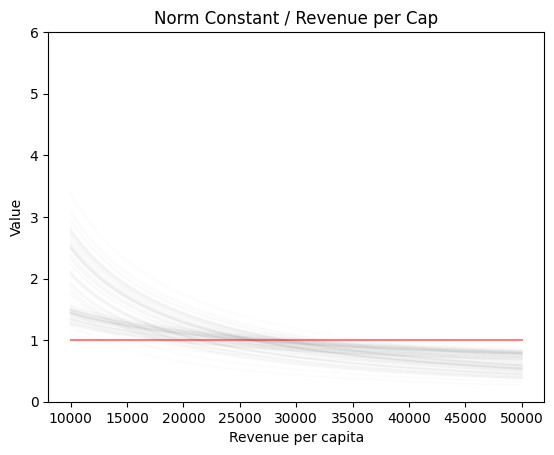
\includegraphics[width=0.75\linewidth]{figures/coef.png}

\end{methodbox}
\begin{methodbox}[Execution des différents runs]


    
\end{methodbox}

\subsection{Modèle économétrique}

On construit un modèle économétrique dont la forme générale est la suivante : 


\begin{align}
\label{eq:modele}
    \text{Niveau de dommage} = & \ \beta_0  + \underbrace{\beta_1 \cdot \text{temperature}}_\text{Variables physiques}  + \underbrace{\beta_3 \cdot \text{equation}}_\text{Variables méthodologiques} \\
    & + \underbrace{ \beta_2 \cdot \text{coefficient ethique} + \beta_3 \cdot \text{taux d'actualisation}}_\text{variables éthiques}  + \epsilon
    \end{align}


Les résultats sont plus probants lorsque l'on passe le niveau de dommage au log. Ceci n'a rien d'étonnant. En effet, le modèle a été construit ainsi. En repartant de la manière dont le niveau de dommage est calculé et implémenté dans le dommage, on peut obtenir des équivalences entre ces différentes équations : 

\begin{align*}
& D_{t,r} = f_{dommages} \cdot GDP \cdot \text{coefficient éthique}\\
\iff & D_{t,r} = f(\text{temperature}, \text{ autres facteurs})_{t,r} \cdot GDP_{t,r} \cdot \text{coefficient éthique} \\
\iff  & D_{t,r} = \text{temperature}_{t,r}^{\beta_1} \cdot GDP_{t,r}^{\beta_2} \cdot \text{coef}^{\beta_3} \\
\iff & log(D_{t,r}) = log(\text{temperature}_{t,r}^{\beta_1} \cdot GDP_{t,r}^{\beta_2} \cdot \text{coef}^{\beta_3}) \\
\iff & log(D_{t,r}) = \beta_1 \cdot log(\text{temperature}_{t,r}) + \beta_2 \cdot log(GDP_{t,r}) + \beta_3 \cdot log(\text{coef})
\end{align*}
$D_{t,r}$ désigne le niveau de dommage; $f_{dommages}$ désigne la fonction de dommage, qui donne un premier niveau de dommage en fraction du PIB, généralement selon la température.  \\

On obtient ainsi quasiment la forme du modèle économétrique. Ceci peut interroger : en effet, que démontrons-nous, si ce n'est la validité empirique de ces équivalences ? En effet, le pouvoir de démonstration est faible. De toute façon, la causalité ne nous intéresse pas ici :  puisque l'on a \emph{construit} le modèle, on sait de façon certaine la causalité; c'est même une définition. Par ailleurs, on a un contrôle total sur les facteurs qui influencent nos données. En effet, dans les travaux empiriques, les données sont issues de collectes. Elles font l'objet de nombreux biais, et surtout sont influencées par de nombreux facteurs autres que ceux mesurés par le modèle. Ici, on construit ces données, et on peut donc savoir précisément quel facteur influence nos résultats. \\

L'objectif ici n'est pourtant pas de montrer une causalité, mais bien de mesurer l'ampleur de cette variation, et de pouvoir comparer les impacts des différents facteurs. Les régressions permettent de synthétiser ces variations en des coefficients uniques, \emph{ceteris paribus}.

L'objectif est de quantifier l'impact relatif des variables physiques, méthodologiques et éthiques. On réalise ensuite cinq régressions linéaires, qui sont des variations du modèle présenté plus haut. 


On a d'abord une régression simple du niveau de dommage selon la température : 

\begin{align}
\text{Niveau de dommage} = & \ \beta_0  + \beta_1 \cdot \text{temperature}  + \epsilon
\end{align}

Cette première étape nous permet de comparer les résultats de nos modèles plus complexe avec un modèle plus simple, pour s'assurer que prendre en compte les autres facteurs apporte effectivement un pouvoir explicatif complémentaire.  \\

On ajoute ensuite le coefficient éthique, sans tenir compte à ce stade de la forme de l'équation ni contrôler par la région. 

\begin{align}
\text{Niveau de dommage} = & \ \beta_0  + \beta_1 \cdot \text{temperature}  + \beta_2 \cdot \text{coefficient ethique} + \epsilon
\end{align}

On cherche maintenant à observer l'effet de la forme de la fonction de dommage : 

\begin{align}
\text{Niveau de dommage} = & \ \beta_0  + \beta_1 \cdot \text{temperature}  + \beta_3 \cdot \text{equation} + 
 \beta_2 \cdot \text{coefficient ethique} + \beta_3 \cdot \text{taux d'actualisation}  + \epsilon
\end{align}

On essaie également de contrôler les différences régionales en tenant compte de celles-ci grâce à une dummy. 

\begin{align}
\text{Niveau de dommage} = & \ \beta_0  + \beta_1 \cdot \text{temperature}  + \beta_2 \cdot \text{coefficient ethique} + \beta_3 \cdot \text{région} + \epsilon
\end{align}

Finalement, le modèle le plus complet prend en compte à la fois la température (variable physique), l'équation (variable méthodologique) et le coefficient éthique (variable éthique), tout en contrôlant par les régions. 
\begin{align}
\text{Niveau de dommage} = & \ \beta_0  + \beta_1 \cdot \text{temperature}  + \beta_2 \cdot \text{coefficient ethique} + \beta_3 \cdot \text{région} + \beta_4 \cdot \text{équation} + \epsilon
\end{align}
\paragraph{Evaluation de l'estimateur} \cite{wooldridge_introductory_2016} propose 5 critères pour un bon estimateur. D'abord, on doit écrire notre modèle économétrique sous la forme d'une combinaison linéaire des variables explicatives. C'est bien le cas ici (voir équation \ref{eq:modele} Ensuite, l'échantillon doit être aléatoire. Dans notre cas, nous avons fait varier de manière aléatoire les paramètre du modèle; on observe néanmoins des schémas dans la distribution des valeurs des niveaux de dommage; il est donc possible que cet échantillon ne soit pas tout à fait aléatoire. Cela s'expliquerait par exemple par des différences systématiques liées à la région (on observe d'ailleurs que lorsque l'on contrôle par la région, cet effet disparait).  Il faut ensuite avoir une variation des échantillons, ce qui est notre cas. Puis, il faut que l'espérance conditionnelle des termes d'erreur soit nulle. On observe bien cela ici. En revanche, les tests d'homoscédasticité montrent qu'il y a de l'hétéroscédasticité.  Ces différentes analyses sont développées sur le site \blog{https://damage-functions-modeling.readthedocs.io/en/latest/3_modelling/regprep.html}.

\begin{figure}
    \centering
    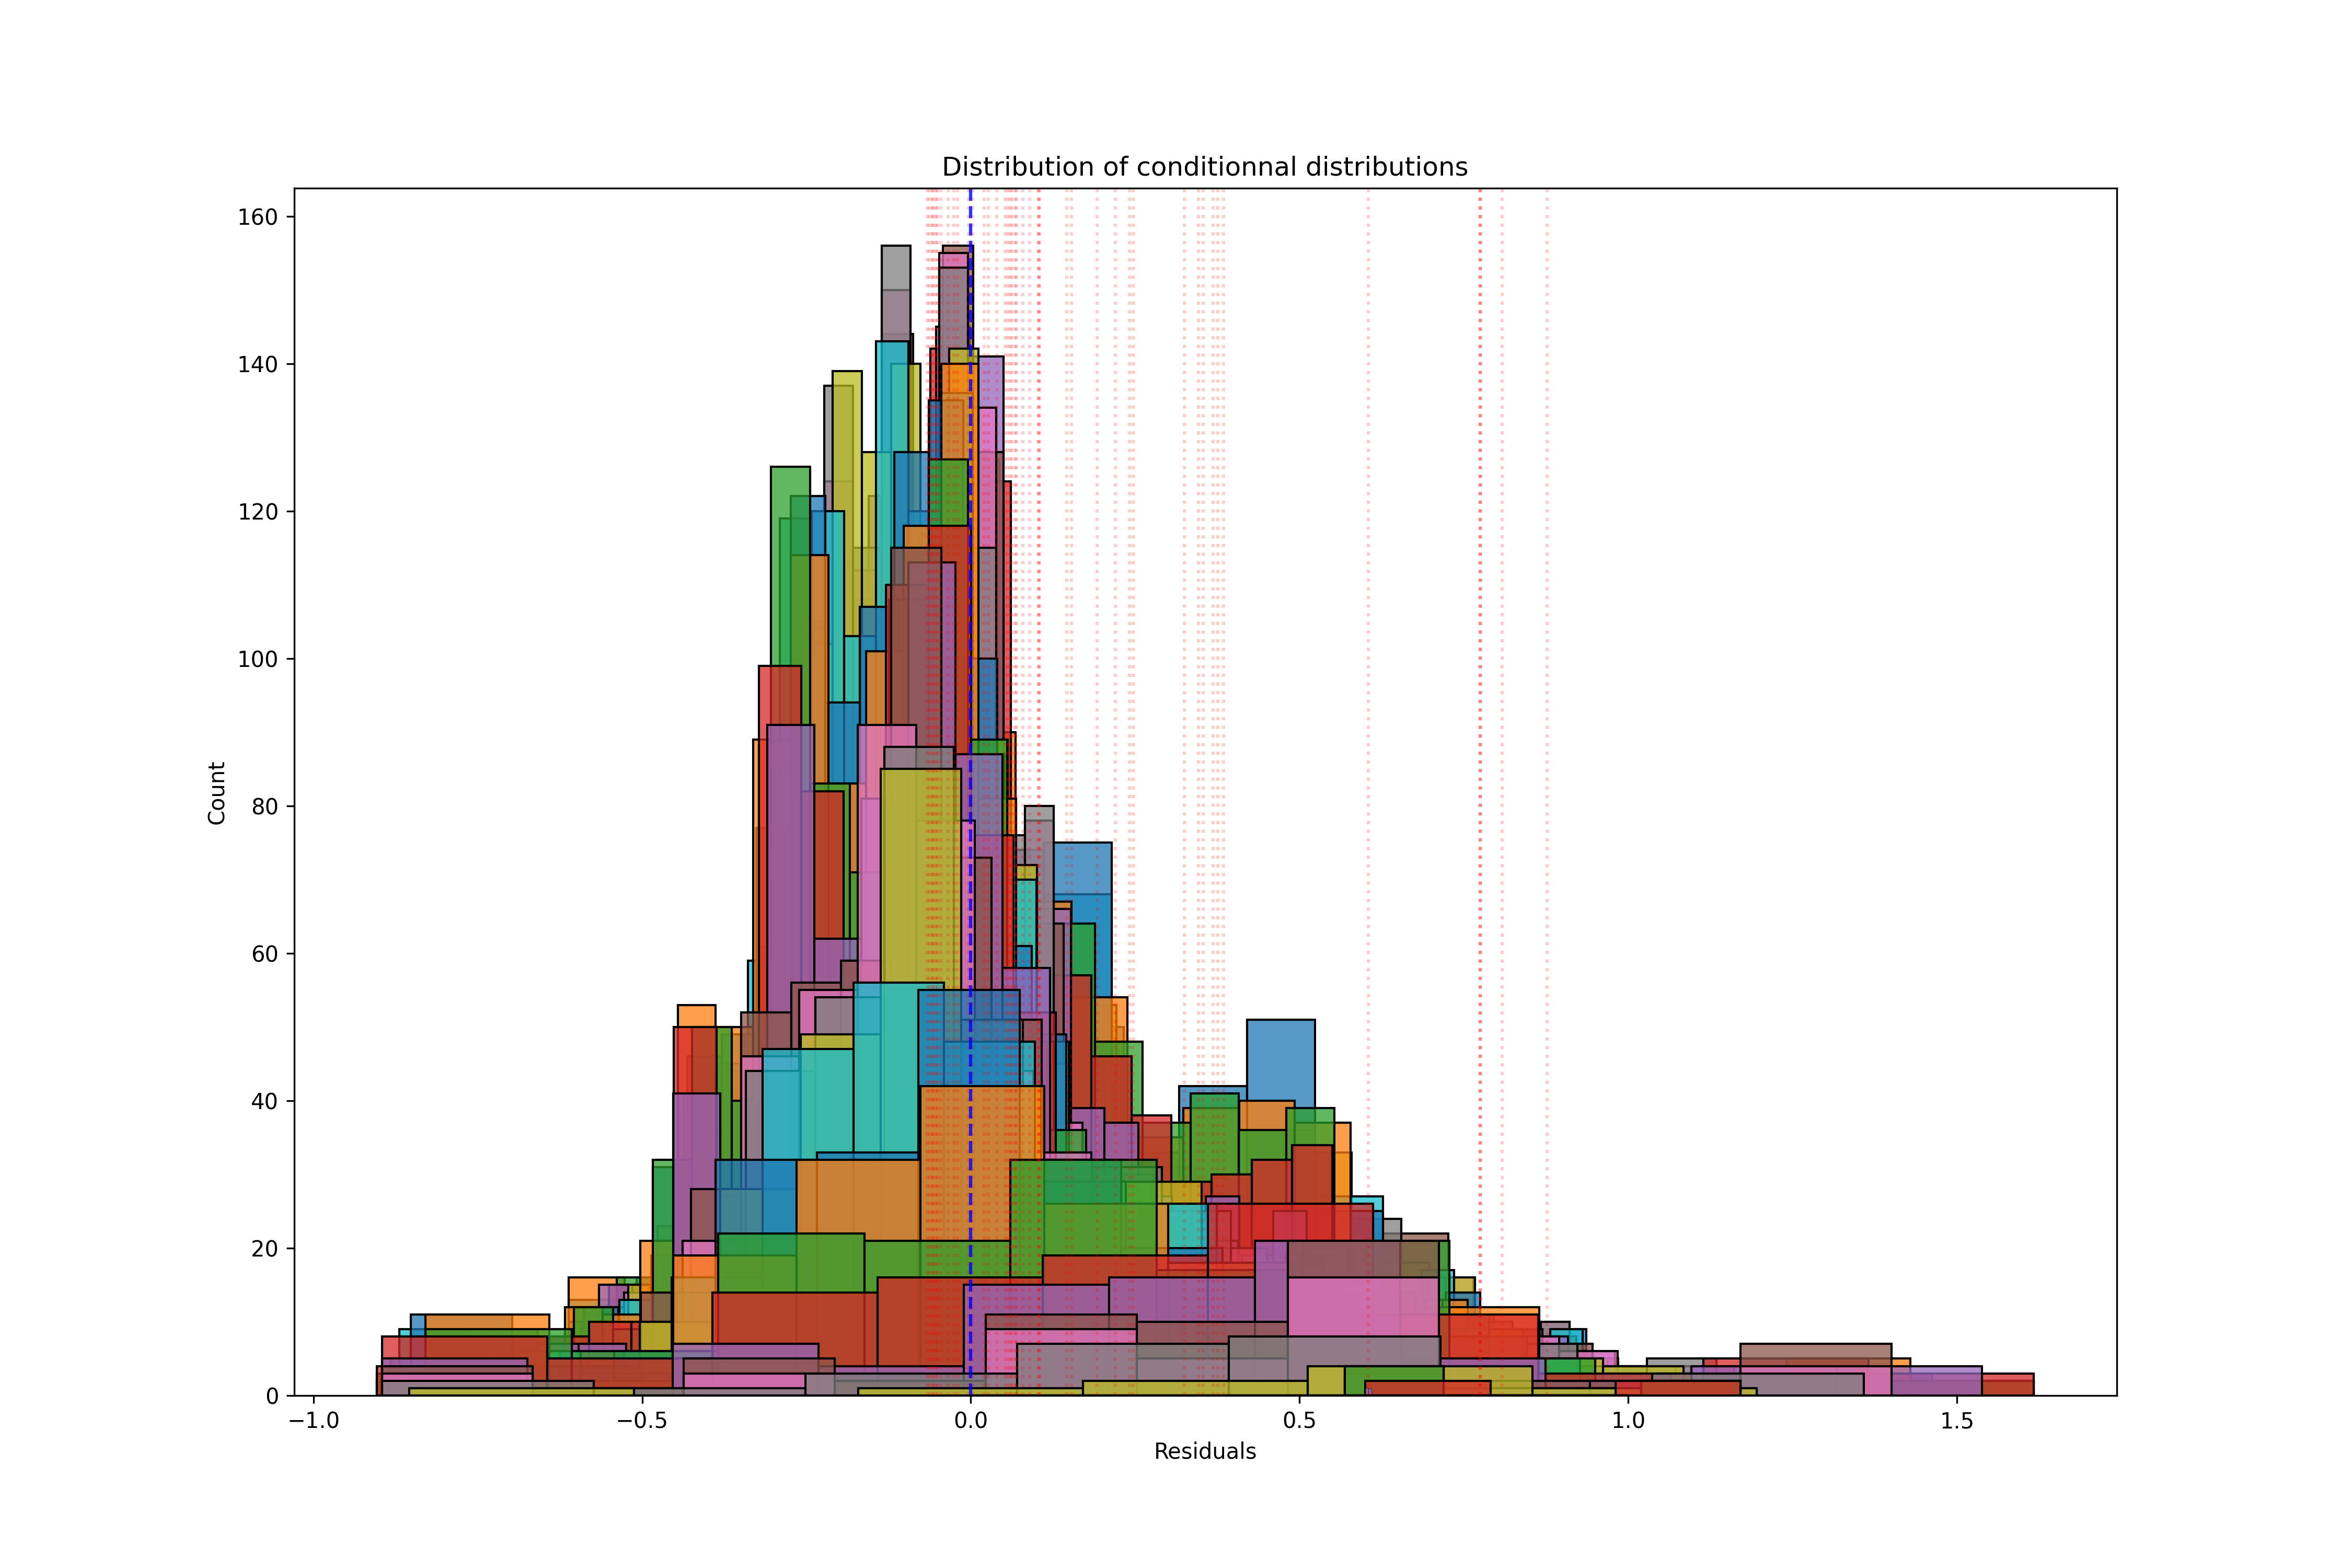
\includegraphics[width=\linewidth]{results/slr_4_2.png}
    \legende{Espérence conditionnelle des termes d'erreurs}{Cette figure représente la distribution des espérences des termes d'erreurs selon plusieurs  des conditions sur la variable explicative $x$. Cela signifie qu'il n'y a pas trop d'erreur systématique selon la valeur  de la variable explicative. On remarque néanmoins que la forme n'est pas symmétrique, avec des erreurs fortement négatives. }
    \label{fig:slr_4}
\end{figure}

L'échantillon ne respect pas les cinq critères de Wooldridge. De ce point de vue, on peut penser que ce n'est pas un très bon estimateur, et qu'il faut chercher à améliorer notre modèle. Cependant, nous ne cherchons pas ici à avoir un pouvoir explicatif, mais bien à avoir une mesure quantitative d'un phénomène dont on sait qu'il existe, puisque nous l'avons définit ainsi. 


\begin{methodbox}
On utilise ici le modèle WILIAM. Il s'agit d'un modèle open source, donc il est assez facile de le répliquer, modifier et distribuer. Le code source est disponible sur Github. On réalise une fork du code source, c'est-à-dire une branche de code. Notre branche de code devient un projet autonome sur lequel on peut travailler de manière semi-indépendante du projet. En effet, les modifications du projet WILIAM ou celles réalisées ici ne s'affecteront pas, à moins que l'on push notre code vers le code principal, ou que l'on pull les nouvelles modifications du code principal vers notre branche. Ces deux opérations peuvent se faire sous supervision, pour s'assurer que l'on n'interagit pas avec différentes parties de notre code, ce qui risquerait de fausser nos résultats. \blog{https://damage-functions-modeling.readthedocs.io/en/latest/3_notebooks/spatial_temporal_equity.html} \\

Dans cette branche, on modifie le code pour qu'il représente les fonctions de dommage. On modélise ainsi plusieurs formes de fonctions de dommage, issues de la revue de littérature évoquée plus haut. On fait tourner le modèle avec ces différentes fonctions de dommage, et en faisant varier aléatoirement les différents paramètres : taux d'actualisation, les différents paramètres qui entrent en compte dans le modèle. \\

On récupère les résultats et on procéde à des analyses économétriques sur les résultats pour voir quels sont les paramètres qui ont le plus influencé les résultats. La largeur de la page est \the\textwidth. En centimètres, cela donne \uselengthunit{cm}\printlength{\textwidth}.

\end{methodbox}

\begin{figure}
    \centering
    \begin{overpic}[width=\linewidth]{illustrations/methodo_econometrie.png}
        \put(10, 90){WILIAM}
        %\put(50,70){\Huge $E=mc^2$} % Texte au centre de l'image
        %\put(10,20){\color{red}\huge Important} % Texte en bas à gauche
    \end{overpic}
    %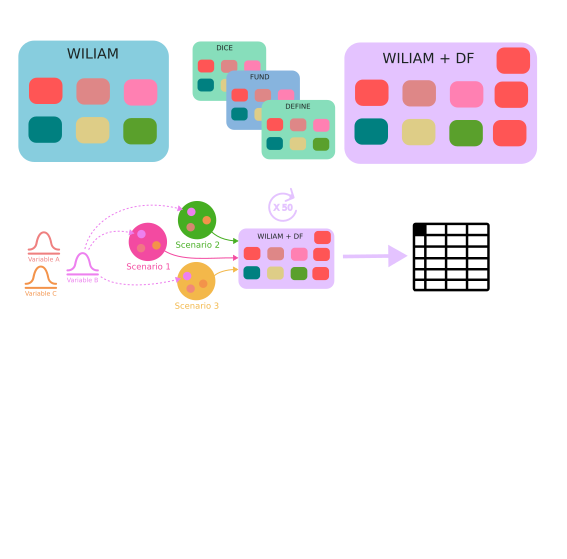
\includegraphics[width=0.9\textwidth]{illustrations/methodo_econometrie.png}
    \legende{Méthodologie de la comparaison des modèles. (SVG)}{On utilise le modèle open-source WILIAM. Celui ci est composé de différents modules, dont un module représentant les dommages (représenté ici en rouge). On identifié les fonctions de dommage d'autres modèles (DICE, FUND et DEFINE). On les isole, et on les implémente dans le modèle WILIAM. On a alors un nouveau modèle, qui contient simultanément plusieurs manières de représenter les dommages. On connait la distribution de certains paramètres, et on cherche à voir l'effet de cette variation sur les résultats du modèle. On réalise des scénarios, qui sont des combinaisons de tirage aléatoire des variables. Le modèle est executé avec chaque scénario, de nombreuses fois. Tous ces \textit{runs} forment une grande base de donnée, sur laquelle on va réaliser une étude économétrique. }
    \label{fig:methodo-simu}
\end{figure}

\subsection{Limites et contraintes}

Plusieurs limitations doivent être soulignées. 

\paragraph{Transposition dans un autre modèle} D'abord, on utilise les fonctions de dommage de différents modèles dans le modèle WILIAM. Cela permet d'avoir les même conditions pour toutes les fonctions de dommage. Ceci étant dit, les fonctions ne sont plus dans leur milieu d'origine. Ceci pose deux problème. D'abord, les fonctions peuvent avoir été calibrées pour fonctionner correctement dans certaines conditions de fonctionnement de température, et pas au delà; et ces conditions peuvent ne pas être atteinte dans WILIAM. Cela est notamment vrai pour toutes les variables qui nécessitent une calibration, par exemple celles où la population entre en jeux. Une population différente peut aboutir à une fonction de dommage qui est différente. Ensuite, il y a un grand risque d'erreur de transcription. En effet, les variables peuvent avoir les mêmes noms mais ne pas désigner la même chose précisement ou ne pas être calculée de la même manière; ou encore, la documentation d'origine peut ne pas être claire sur les caractéristiques précises d'une variable (notamment, le niveau de désagrégation). On peut néanmoins considérer que ce n'est pas une limitation très forte. En effet, nous nous intéressons ici à la \emph{relation} entre les hypothèses et le niveau de dommage, et pas au niveau de dommage \emph{en soi}. Ainsi, une mauvaise calibration risque de donner des valeurs trop faibles ou trop élèvées, mais n'a pas d'effet sur la relation en soi. Par ailleurs, ces fonctions sont justement présentées comme des relations liant les phénomènes climatiques à un niveau de dommage. Si changer de modèle affecte grandement la validité de la relation, alors on peut interroger la validité de la relation dans son ensemnle. 

\paragraph{Collinéarité} Le problème majeur de cette technique est que les données analysées ont été produites dans la perspective de cette analyse. Ainsi, il est possible que le résultat de l'analyse de reflète que les hypothèses et les variations qui ont été volontairement ajoutées au modèle. En particulier, le niveau de dommage dépend beaucoup de la valeur du coefficient d'éthique spatial, qui est lui même construit pour l'expérience. 



\section{Résultats}





\subsection{Inégalités temporelles}


\subsection{Inégalités spatiales} 

\begin{landscape}
    \begin{table}\resizebox{\textwidth}{!}{%
\centering
\begin{tabular}{@{\extracolsep{5pt}}lcccc}
\\[-1.8ex]\hline
\hline \\[-1.8ex]
& \multicolumn{4}{c}{\textit{Dependent variable: log\_damage}} \
\cr \cline{2-5}
\\[-1.8ex] & \multicolumn{1}{c}{Temp} & \multicolumn{1}{c}{Equation} & \multicolumn{1}{c}{Country} & \multicolumn{1}{c}{Double}  \\
\\[-1.8ex] & (1) & (2) & (3) & (4) \\
\hline \\[-1.8ex]
 Temperature Change & 2.840$^{***}$ & 2.837$^{***}$ & 2.864$^{***}$ & 2.864$^{***}$ \\
& (0.009) & (0.007) & (0.002) & (0.002) \\[2em]
 log\_coef & & 1.000$^{***}$ & 1.003$^{***}$ & 1.003$^{***}$ \\
& & (0.004) & (0.001) & (0.001) \\[2em]
 DICE form damage function & & -0.196$^{***}$ & & -0.196$^{***}$ \\
& & (0.010) & & (0.003) \\[2em]
 WITNESS form damage function & & 0.350$^{***}$ & & 0.350$^{***}$ \\
& & (0.010) & & (0.003) \\[2em]
 Regional dummy & No & No & Yes & Yes \\
\hline \\[-1.8ex]
 Observations & 231378 & 231378 & 231378 & 231378 \\
 $R^2$ & 0.315 & 0.492 & 0.955 & 0.962 \\
 Adjusted $R^2$ & 0.315 & 0.492 & 0.955 & 0.962 \\
 Residual Std. Error & 2.209 (df=231376) & 1.903 (df=231373) & 0.566 (df=231353) & 0.519 (df=231351) \\
 F Statistic & 106536.752$^{***}$ (df=1; 231376) & 55991.215$^{***}$ (df=4; 231373) & 204959.303$^{***}$ (df=24; 231353) & 226667.979$^{***}$ (df=26; 231351) \\
\hline
\hline \\[-1.8ex]
\textit{Note:} & \multicolumn{4}{r}{$^{*}$p$<$0.1; $^{**}$p$<$0.05; $^{***}$p$<$0.01} \\
\end{tabular}
}\end{table}
\end{landscape}


\begin{table}\resizebox{\textwidth}{!}{
    \centering
      
\begin{tabular}{@{\extracolsep{5pt}}lccc}
\\[-1.8ex]\hline
\hline \\[-1.8ex]
& \multicolumn{3}{c}{\textit{Dependent variable: log\_damage}} \
\cr \cline{2-4}
\\[-1.8ex] & \multicolumn{1}{c}{Temp} & \multicolumn{1}{c}{Simple} & \multicolumn{1}{c}{Equation}  \\
\\[-1.8ex] & (1) & (2) & (3) \\
\hline \\[-1.8ex]
 Temperature Change & 4.083$^{***}$ & 4.110$^{***}$ & 4.110$^{***}$ \\
& (0.027) & (0.025) & (0.024) \\[2em]
 Exponent (log) & & 0.188$^{***}$ & 0.188$^{***}$ \\
& & (0.011) & (0.011) \\[2em]
 Constant (log) & & -0.683$^{***}$ & -0.683$^{***}$ \\
& & (0.030) & (0.029) \\[2em]
 DICE form damage function & & & -0.202$^{***}$ \\
& & & (0.031) \\[2em]
 WITNESS form damage function & & & 0.344$^{***}$ \\
& & & (0.031) \\[2em]
\hline \\[-1.8ex]
 Observations & 5073 & 5073 & 5073 \\
 $R^2$ & 0.824 & 0.847 & 0.856 \\
 Adjusted $R^2$ & 0.824 & 0.847 & 0.856 \\
 Residual Std. Error & 0.997 (df=5071) & 0.928 (df=5069) & 0.901 (df=5067) \\
 F Statistic & 23720.751$^{***}$ (df=1; 5071) & 9378.777$^{***}$ (df=3; 5069) & 6041.199$^{***}$ (df=5; 5067) \\
\hline
\hline \\[-1.8ex]
\textit{Note:} & \multicolumn{3}{r}{$^{*}$p$<$0.1; $^{**}$p$<$0.05; $^{***}$p$<$0.01} \\
\end{tabular}
 
    \legende{Résultats des régressions aggrégées par pays}{}
    \label{tab:reg_glob}
}\end{table}


\begin{figure}
    \centering
    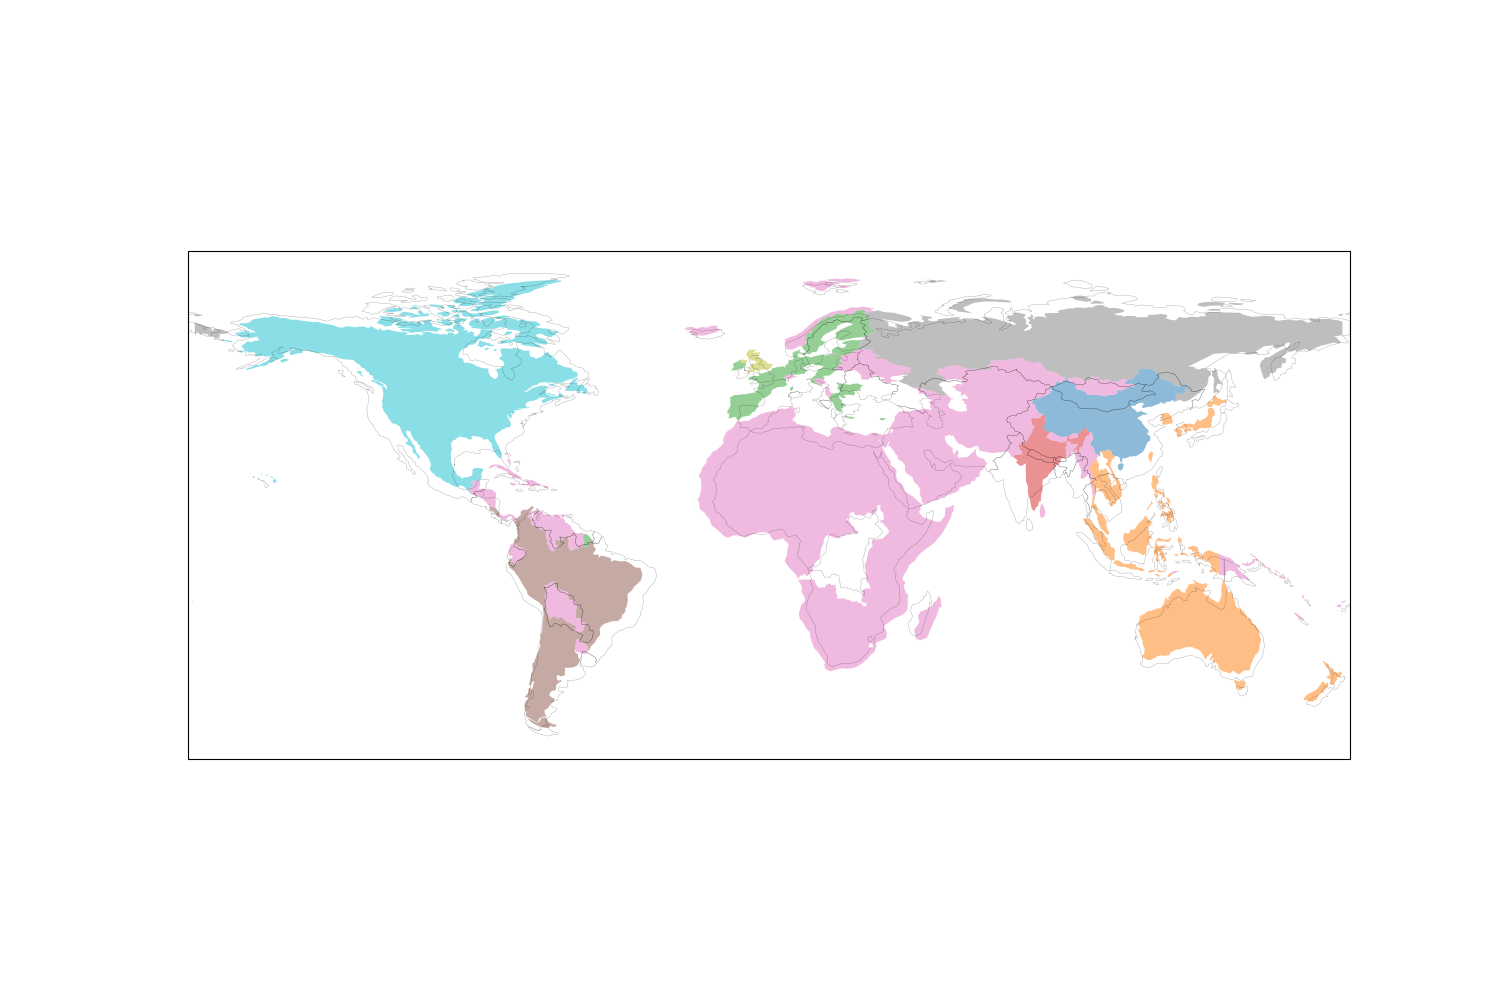
\includegraphics[width=\linewidth]{results/cartogramme.png}
    \legende{Carte en anamorphose selon le niveau de dommage}{Cette carte déforme l'espace pour que la surface de chaque zone soit proportionnelle à la valeur absolue des dommages subis.}
    \label{fig:anamorphose}
\end{figure}

\begin{figure}
    \centering
    %\includegraphics[width=0.5\linewidth]{}
    \legende{Les dommages selon la manière de comptabiliser le revenu par habitants}{}
    \label{fig:carte1}
\end{figure}
\subsection{Inégalités sociales}


\begin{figure}
    \centering
    %\includegraphics{}
    \legende{Coûts des dommages selon la fonction de dommage incluse dans le modèle WILIAM.}{Graphiques représentant la valeur totale des dommages dans le modèle WILIAM selon la fonction de dommage. Les couleurs représentant le modèle d'origine de la fonction de dommage; la ligne pleine la médiane, la zone grisée les valeurs interquartiles.}
    \label{fig:simu}
\end{figure}


\section{Discussion}

\subsection{Interprétation des résultats}

%Que signifient vos résultats par rapport à vos hypothèses ? Quelles conclusions pouvez-vous en tirer ? 

\subsection{Comparaison avec la littérature}
% Comment vos résultats s'intègrent-ils dans le contexte de la littérature existante ? Confirment-ils ou remettent-ils en question les résultats antérieurs ? 

\subsection{Implications pratiques}
% Quels sont les impacts ou les applications potentielles de vos résultats dans le domaine étudié ? 

\subsection{Limites}
%Quelles sont les limitations de votre étude ? Cela peut concerner des problèmes méthodologiques, des échantillons insuffisants, etc 

\subsection{Perspectives futures}
% Quelles recherches supplémentaires pourraient être nécessaires pour approfondir vos découvertes ou explorer des questions connexes ?
\chapter{Éthique de la modélisation intégrée}
\label{chapter:ethique}
\newrefsegment

\PEEL{Les modélisateur.ices ont une responsabilité vis à vis de ce que leurs modèles produisent. }{Fournissez des preuves, des données ou des citations qui soutiennent votre point.}{Expliquez en quoi les preuves que vous avez fournies sont pertinentes et comment elles appuient votre point.}{Faites le lien avec le sujet principal ou avec la section suivante de votre mémoire.}


\chapterabstract{Les choix de modélisation des fonctions de dommage sont lourds de conséquences sur le message que véhiculent les résultats de ces modèles. Ces résultats alimentent le débat public sur les questions climatiques. Vu les enjeux sociaux et sociétaux qui sont à l'oeuvre, la pratique de la modélisation implique des questions éthiques importantes. Quelles sont-elles, et comment sont-elles prises en compte ? Cette partie est plus conceptuelles et épistémiques, et cherche à identifer des points d'attention de la modélisation.}

\begin{quote}
    Dépolitiser le réel c'est le repolitiser au profit de l'oppresseur
\end{quote}


\begin{table}
    \centering
    \begin{tabular}{|c|c|c|c|} \hline 
         Pratique&  Enjeu&  Concept associé& Commentaire\\ \hline 
         Choisir les modèles pour faire tourner les scénarios&  Framing / possibility space&  & \\ \hline 
         Attribuer une valeur à un paramètre (taux d'actualisation)&  Equité intergénérationnelle&  & \\ \hline 
         Fabrique du doute&  Responsabilité dans l'interprétation des résultats&  Doute normativement inappropriés& \\ \hline
    \end{tabular}
    \legende{Enjeux éthiques dans les modèles et cadre d'analyse associés}{}
    \label{tab:ethique}
\end{table}


\cite{schienke_intrinsic_2011} => sur l'éthique intrinsèque dans les IAMs
\cite{weitzman_modeling_2009} => sur les evenements non-linéaires

\begin{tcolorbox}
    Voir Gouverner le climat !!
\end{tcolorbox}


\section{Les trois niveaux de l'éthique et la responsabilité du modélisateur}

Cette section pose plusieurs questions quant à la place de la technique et de la modélisation dans la cité. 

Elle s'appuie notamment sur \cite{jonas_principe_2008} et \cite{vast machine}, ainsi que sur la classification des enjeux éthiques de \cite{tuana_leading_2010}.


Comme nous l'avons vu précédemment, le processus de modélisation est avant tout un processus de sélection de ce qui est représenté et ce qui ne l'est pas, et de décision de la manière de le représenter. Comme nous le verrons dans le chapitre \ref{chapter:socio}, l'imperfection et la partialité des modèles est souvent assumée, voire revendiquée par les équipes de modélisation. Elle s'accompagne souvent d'une tentative de dé-responsabilisation de l'équipe de modélisation. Celle-ci prend généralement la forme suivante : 

\begin{quote}
    Les résultats des modèles sont valables uniquement sous les conditions (nombreuses et irréalistes) dans lesquelles il a été conçu. On ne peut donc pas extrapoler les résultats, ou faire dire au modèle autre chose que ce qu'il veut dire. 
\end{quote}
Pourtant, les résultats des modèles sont utilisés de manière large, notamment pour prendre des décisions de politique publique, y compris par des personnes n'ayant pas de compétence spécifique en modélisation, ni de connaissance particulière des modèles utilisés pour produire les connaissances qu'elles utilisent. Il y a donc un paradoxe : d'une part, l'idéal d'une compréhension fine des hypothèses de la modélisation, qui permet d'être conscient des choix de modélisation et de leurs implications. Cet idéal protège la responsabilité du modélisateur : en effet, les hypothèses ayant été clairement formulées, l'utilisateur final devient responsable de sa propre interprétation. Celle-ci se fait en accord avec les hypothèses énoncées, que l'utilisateur final fait sienne. D'autre part, il est difficile de comprendre un modèle pour plusieurs raisons : technique (les logiciels ne sont pas/plus accessibles), légales (le code source n'est pas accessible librement), capacitaires (les codes sources sont difficiles à interpréter, surtout si on n'est pas familier du langage utilisé), théoriques (les modèles intégrés font appel à des concepts issus de nombreuses disciplines). Cette difficulté à comprendre les modèles font que les résultats sont \textit{de facto} souvent interprétés dans l'état dans lequel ils sont délivrés, sans la contextualisation permise par le code. Dès lors, le choix des hypothèses est invisibilisé, et la responsabilité du modélisateur peut s'étendre jusqu'à l'interprétation du modèle, voire jusqu'aux conséquences de cette interprétation. \\

Pour éclairer ce paradoxe, nous allons nous intéresser aux dimensions éthiques de la modélisation. Pour cela, nous allons nous appuyer sur les travaux de Tuana, qui a cherché à developper un cadre conceptuel de l'éthique dans la recherche, et qu'elle a adapté spécifiquement au cas de la modélisation intégrée. \\

Elle développe trois dimensions éthiques de la recherche scientifique : l'éthique procédurale, l'éthique intrinsèque et l'éthique extrinsèque. 

\begin{figure}
    \centering

    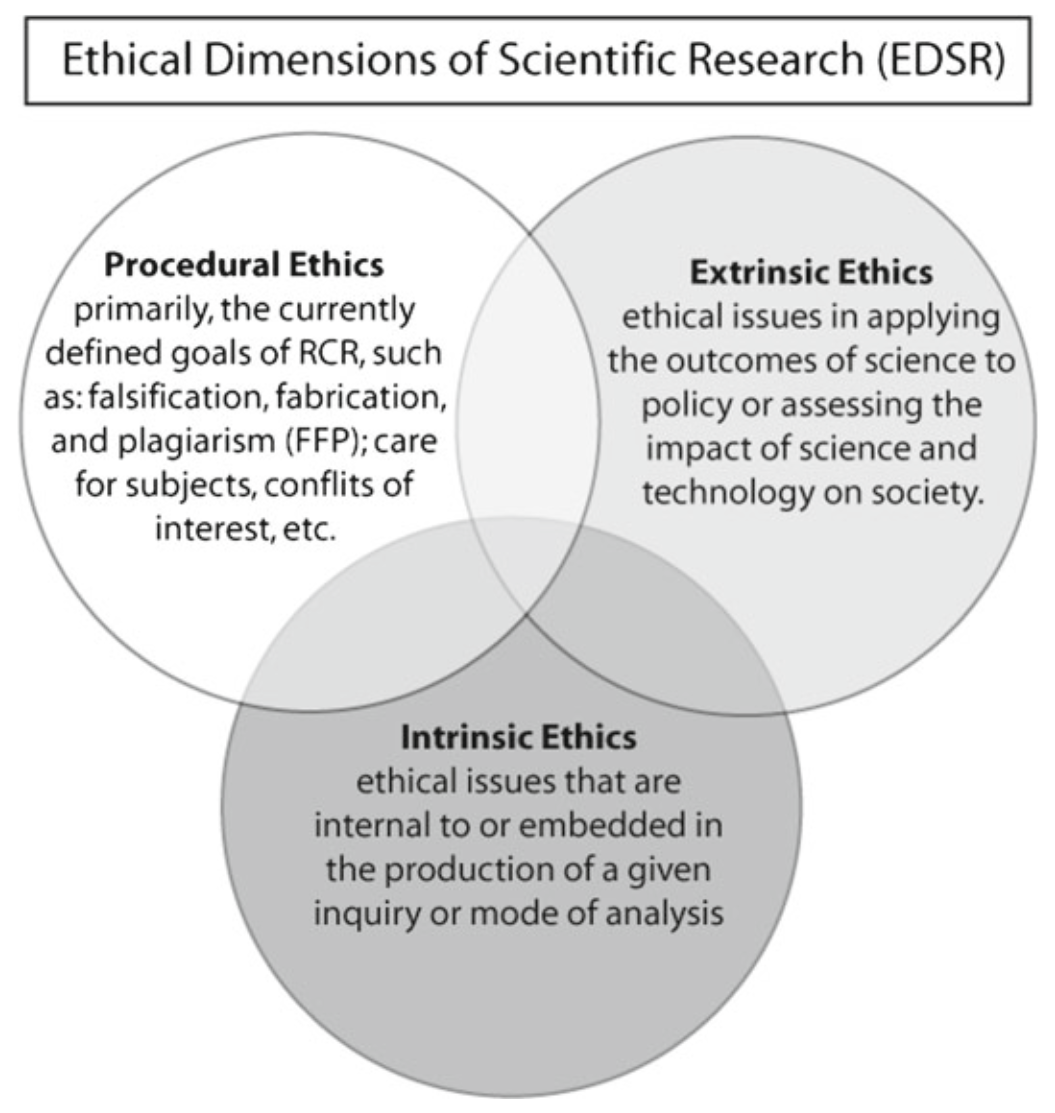
\includegraphics[width=1\linewidth]{venn_ethics.png}
    \legende{Les trois dimensions de l'éthique dans la recherche.}{\cite{tuana_climate_2019} décrit trois dimensions éthiques dans la recherche : l'éthique procédurale consiste en le respect des normes établies et reconnues dans la communauté. C'est en général ce à quoi on fait référence quand on parle de \textit{bonne science}. L'éthique extrinsèque désigne les questions éthiques qui sont liées aux utilisations des productions scientifiques. Enfin, l'éthique intrinsèque désigne les questions qui sont incluses dans le mode de production de la connaissance (en l'occurence, le modèle). }
    \label{fig:diag-venn}
\end{figure}


\subsection{L'éthique procédurale}

L'\Gls{procedural ethics} désigne ce qui est couramment regroupé sous le terme de \textit{bonne science}, ou \textit{good science}. Il s'agit de produire de la connaissance en respectant les attentes de la communauté scientifique en termes de honneteté, de sincérité. Tuana \cite{tuana_leading_2010}  la définit comme ceci : 

\begin{quote}
Ethical aspects of the process of conducting scientific research, such as: falsification, fabrication, and plagiarism; care for subjects (human and non-human animal); responsible authorship issues; analysis of and care for data.
\end{quote}
La plupart des travaux de modélisation s'inscrivent pleinement dans cette démarche, et sont en phase avec les attentes et bonnes pratiques de la communauté : 

\begin{itemize}
    \item tranparence : les codes sources sont ouverts et accessible, il y a une documentation plus ou moins complète
    \item honneteté : les hypothèses sont clairement énoncées
    \item sincérité des résultats : les résultats sont reproductibles facilement
\end{itemize}

\begin{tcolorbox}
    Mais remarques de Keen sur Nordhaus
\end{tcolorbox}

\subsection{L'éthique intrinsèque}

L'\Gls{intrinsic ethics} va plus loin dans l'exigence. Il s'agit de la dimension éthique qui est directement intégrée dans le processus de recherche : il ne s'agit plus de la forme de la recherche, mais du fond de la recherche. 

\begin{quote}
Ethical issues and values that are embedded in or otherwise internal to the production of scientific research and analysis. These involve ethical issues arising from, for example: the choice of certain equations, constants, and variables; analysis of data; handling of error, and degree of confidence in projections.
\end{quote}
Comme le souligne Tuana, la bonne prise en compte de ces questionnements nécessite d'avoir un accompagnement épistémologique au sein des équipes de recherche, c'est-à-dire de prendre en compte ces enjeux comme partie intégrante du développement du projet : \emph{the domain of intrinsic ethics will not be fully successful unless it includes the expertise of philosophers of science. It is only when this domain becomes a focus of our field, that the range of relevant issues and their ethical and epistemic significance will be fully appreciated.} 

\begin{tcolorbox}
    A développer : 
    \begin{itemize}
        \item choix du taux d'actualisation
        \item 
    \end{itemize}
\end{tcolorbox}

Un exemple d'éthique intrinsèque est le découpage par région. Les modèles se focalisent sur certaines régions plus que d'autres, sont calibrés sur certaines régions (où il y a par ailleurs des données plus nombreuses et de meilleure qualité), et sont donc bien plus pertinents pour décrire les phénomènes dans certaines régions plus que dans d'autres. 

\begin{figure}[htbp]
    \centering
    \begin{minipage}{0.45\textwidth}
        \centering
        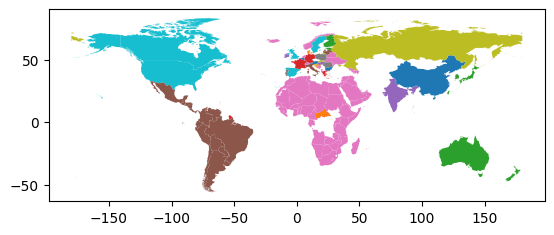
\includegraphics[width=\linewidth]{figures/FUND_regions.png} % Remplacez par le chemin de votre image
        \subcaption{FUND}
        \label{fig:carte1}
    \end{minipage}%
    \hfill
    \begin{minipage}{0.45\textwidth}
        \centering
        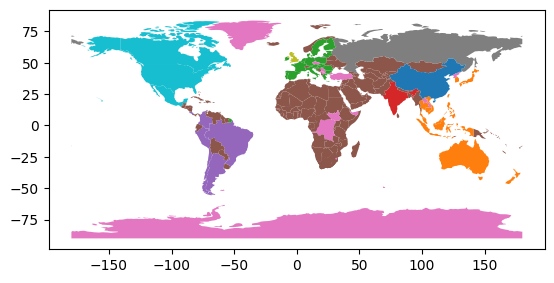
\includegraphics[width=\linewidth]{figures/WILIAM_regions.png} % Remplacez par le chemin de votre image
        \subcaption{WILIAM}
        \label{fig:carte2}
    \end{minipage}%
    \legende{Granularité spatiale différente entre les modèles}{}
    \label{fig:trois_cartes}
\end{figure} 



\subsection{L'éthique extrinsèque}

Enfin, l'\Gls{extrinsic ethics} désigne les questionnements autour des effets de la production scientifique sur la société. C'est une sphère beaucoup plus large, puisqu'elle sort du domaine du laboratoire et de la communauté scientifique, pour mesurer les effets sur les sociétés. 

\begin{quote}
Ethical issues that are external to the production of scientific research. These arise, for example, when considering the impact of scientific research on society; e.g., the effects of technological innovations on social ends such as health and well-being, whether pressing social and economic issues are likely to be addressed and if so, who benefits, and the role of science in policy-making. This domain of ethics also includes ethical concerns arising from the impact of society upon science, for example the impact of funding on research trajectories or the ways in which wide-spread societal biases can impact research trajectories, as they arguably did with eugenics research. In the latter case, there are often links between the domains of extrinsic and intrinsic ethics.
\end{quote}
Ce questionnement s'inscrit dans une réflexion plus large du rapport entre la production scientifique et son application dans la société. 

\begin{tcolorbox}
\begin{itemize}
    \item 
    \item [[cadrage]], forcément normatif « IAM analysis could focus on only a subset of relevant futures and thus push society in certain directions without sufficient scrutiny » (\href{zotero://select/library/items/2SDDNUUF}{“Annex III: Scenarios and Modelling Methods”, 2023, p. 1862}) (\href{zotero://open-pdf/library/items/CHVFSLLH?page=22&annotation=4MBM5B9Q}{pdf})

\end{itemize}

\end{tcolorbox}


 Ces considérations sur l'éthique extrinsèque prendront plus de sens dans la section suivante, on l'on développera l'idée que la modélisation participe activement au cadrage du débat public, et donc aux choix de futurs possibles. 

\section{Construire / dessiner les futurs possibles}

Cette section montre que le savoir produit par la science est situé dans le temps et dans l'espace. Ainsi, il n'est plus positif, mais bien normatif, en ceci qu'il décrit un univers des possibles. 

Un exemple de à quel point le framing peut impacter la connaissance est la classification des pays. Dans le SPM de l'AR5, les parties n'ont pas pu s'accorder sur un type de classification des pays à adopter ; finalement toutes les figures et textes associés ont été rejetées par les gouvernements. On pourrait ici penser que présenter une information ou une autre n'a pas d'importance, tant que celle-ci a été produite dans les normes scientifiques en vigueur. Pourtant, cet exemple montre que les gouvernements considèrent que le choix d'une classification porte en soi un message trop important ; reconnaissant alors l'absence de neutralité du contenu scientifique \cite{edenhofer_mapmakers_2014}. 

Les modèles intégrés sont utilisés comme base scientifique pour les négociations climatiques. Ils permettent notamment de décrire l'espace des possibles, c'est-à-dire l'ensemble des chemins qui peuvent être pris par les sociétés. Cette relation entre le modèle et la prise de décision est décrite par une image très parlante dans \cite{edenhofer_mapmakers_2014}, où les modélisateurs sont décrits comme des cartographes, et les décideurs comme des navigateurs. Dès lors, le rôle des modélisateurs-cartographe est de décrire l'espace possible, l'ensemble des zones qui sont navigables ; et, si possible, les conditions de navigation que l'on peut rencontrer dans ces zones.  En regard de ces nouvelles connaissances, les décideurs-navigateurs doivent décider du cap à suivre aujourd'hui selon la zone de navigation voulue pour demain. Cette distinction très nette entre décideurs et modélisateurs n'est pas sans limitations. L'une d'entre elle est le cadrage, c'est à dire la manière dont le débat public est façonné par le cadre qu'on lui donne.  Plusieurs choses influencent ce cadrage. Nous verrons d'abord que le prisme technique et énergétique aggrégé de la plupart des modèles représente ce genre de contraintes, sans questionner les modèles sous-jacents. Nous verrons ensuite que le choix des variables, et notamment la monétarisation des dommages fait que de nombreuses dynamiques ne sont soit pas prises en compte, soit prises en compte d'une manière que l'on peut questionner. Enfin, nous, aborderons l'idée que la connaissance est socialement construite, en se basant notamment sur les écrits de Helène Ongino, pour questionner le caractère universel des résultats des modèles. 

\subsection{Un monde homogène, technique et neutre ?}

- Le modèle linéaire de l'expertise
	- « modèle linéaire » ([Aykut et Dahan, 2014, p. 29](zotero://select/library/items/W8P635UZ)) ([pdf](zotero://open-pdf/library/items/LWAJ93IN?
		- « selon lequel la connaissance précède l’application et le consensus scientifique précède l’action politique » ([Aykut et Dahan, 2014, p. 29](zotero://select/library/items/W8P635UZ)) ([pdf](zotero://open-pdf/library/items/LWAJ93IN?pagtation=JCEJGZ8A))
		- « Ce cadrage a pour corollaire la séparation radicale entre science et politique : à la science, les faits, les connaissances ; à la politique, les décisions, les valeurs, les croyances (Proctor, 1991 ; Latour, 1999). » ([Aykut et Dahan, 2014, p. 29](zotero://select/library/items/W8P635UZ)) ([pdf](zotero://open-pdf/library/items/LWAJ93IN?page=otation=D5H6UWJT))
		- « Le cadrage du modèle linéaire est généralement bien accepté, sinon revendiqué, par les scientifiques pour des raisons que l’on peut aisément imaginer : il les protège des intérêts à court terme, d’un pilotage trop étroit par les pouvoirs, les lobbies ou le marché et il semble préserver leur sphère d’autonomie. De plus, cette séparation – si elle était acquise dans les faits – confére rait une légitimité à la science, comme support de l’action politique. » ([Aykut et Dahan, 2014, p. 29](zotero://select/library/items/W8P635UZ)) ([pdf](zotero://open-pdf/library/items/LWAJ93IN?page=otation=DREJ69VN))
	- vs science post-normale (voir becu)
	- « expert » ([Aykut et Dahan, 2014, p. 29](zotero://select/library/items/W8P635UZ)) ([pdf](zotero://open-pdf/library/items/LWAJ93IN?page=ation=BX7ZANJF))
		- « l’adjectif, quand le scientifique expert est un scientifique compétent et familier d’un domaine qu’il a exploré » ([Aykut et Dahan, 2014, p. 29](zotero://select/library/items/W8P635UZ)) ([pdf](zotero://open-pdf/library/items/LWAJ93INation=DVH99DPW))
		- « le substantif, quand l’expert est appelé pour produire, au nom de ses connaissances scientifiques, un avis fondé en vue d’une décision et d’une action politiques » ([Aykut et Dahan, 2014, p. 29](zotero://select/library/items/W8P635UZ)) ([pdf](zotero://open-pdf/library/items/LWAJ93IN?page=notation=87SWXXLB))
	- « Comme le notent Jasanoff et Wynne (1998), la connaissance des experts comporte inévitablement des jugements de valeurs tacites sur la nature et la société. » ([Aykut et Dahan, 2014, p. 29](zotero://select/library/items/W8P635UZ)) ([pdf](zotero://open-pdf/library/items/LWAJ93IN?pageotation=ZH3HKXLT)) 






=> il n'y a pas de modèle qui décompose les dommages par groupe sociaux

Helene Longino va plus loin dans sa critique de la science neutre en s'inscrivant dans une perspective d'épistémologie néo-marxiste. Elle met en avant trois points principaux : les conséquences du progrès technique, qui découle de la science, les travers du réductionnisme, et la possibilité d'une science plus émancipatrice. Cette approche remet les enjeux de rapport de force au cœur de l'épistémologie, et permet d'avoir une lecture politique de la production scientifique. \\

D'abord, elle clame que les dérives du progrès technique sont les inévitables conséquences de la production scientifique. 

\begin{quote}
    One is that the dystopic applications of modern science—the domination of political life by thermonuclear weapons, new particle beam weapons, and other monsters of annihilation; the control of human potentiality through genetic engineering; the proliferation of toxic wastes from science-based technologies; the displacement of human labor by automation—are not a misuse of socially neutral science but the inevitable result of bourgeois science.
\end{quote}

« there are concerns that IAMs are describing transformative change on the level of energy and land use, but are largely silent about the underlying socio-cultural transitions that could imply restructuring of society and institutions » (\href{zotero://select/library/items/2SDDNUUF}{“Annex III: Scenarios and Modelling Methods”, 2023, p. 1862}) (\href{zotero://open-pdf/library/items/CHVFSLLH?page=22&annotation=JY4VBIZY}{pdf})



=> extrait sur le réductionnisme.

\begin{figure}
    \centering
    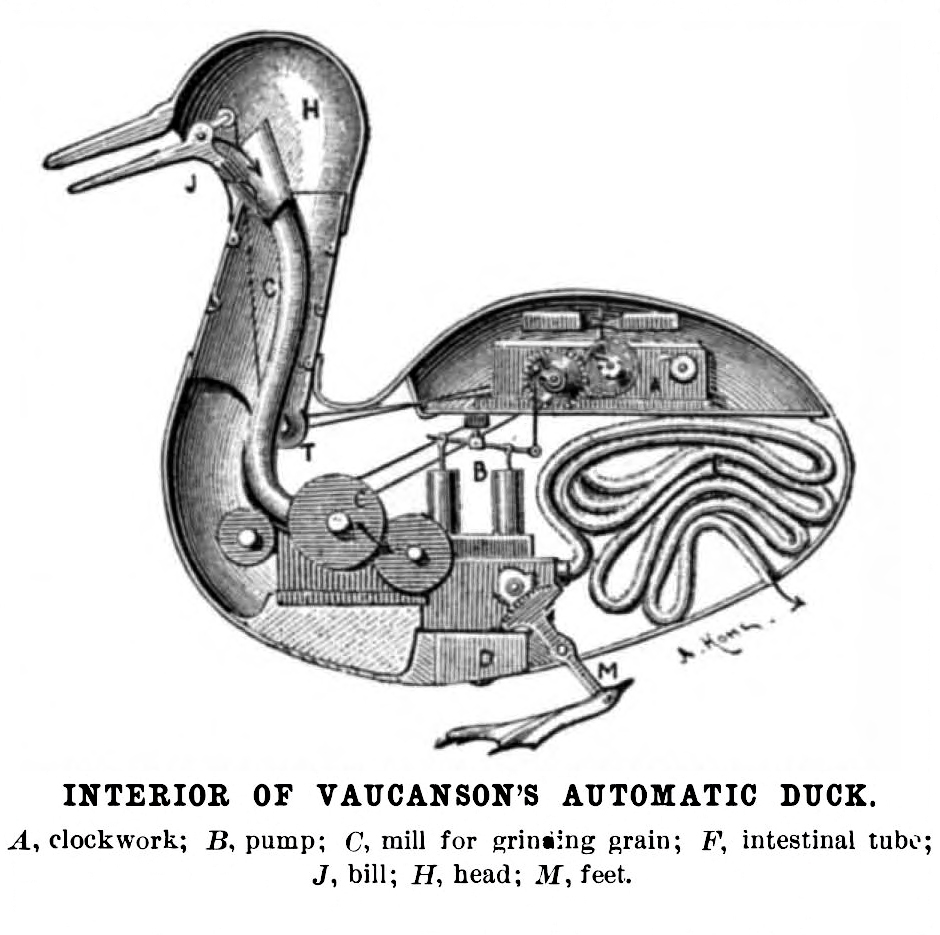
\includegraphics[width=0.75\linewidth]{reductionisme.png}
    \legende{Modèle d'un canard dans une perspective réductioniste}{Le réductionisme tend à décrire les phénomènes par des lois physiques.}
    \label{fig:reductionnisme}
\end{figure}

\begin{quote}
    
\end{quote}

L'autrice continue sa critique en formulant un rejet du réductionnisme, c'est-à-dire à la croyance selon laquelle une notion peut être réduite en d'autres notions plus fondamentales. Elle appelle à une conception plus systémique des des relations causales. 

\begin{quote}
    The spirit, therefore, of these analyses might be better served by seeing them as urging a reconception of objects of inquiry in particular fields — specifically as urging their colleagues to abandon questions presupposing unidirectional or linear causal relations and to understand objects as constituted partly of the parts of which they are wholes and partly of the wholes of which they are parts. If this shift could be accomplished on internalist grounds, there would be less struggle over its acceptance.
\end{quote}

Ce point touche tout à fait les modèles, et particulièrement les fonctions de dommage. Les modèles sont une forme de réductionnisme, puisque l'on représente des phénomènes complexes à travers des fonctions plus simples. Il s'agit donc d'une critique récurrente, mais dont il convient de faire attention. \\


Une autre difficulté rencontrée par les modèles est la représentation des altérités et des différences. Les modèles tendent à décrire un monde homogène et neutralisé. En effet, les régions sont similaires; elles ont certe des paramétrisation différentes, mais les mécanismes décrits sont les mêmes. On gomme par là les différences culturelles et institutionnelles entre les différentes régions du monde. \\

\begin{tcolorbox}
    Partie sur Aykut et Dahan
\end{tcolorbox}

Ces critiques rejoignent celles formulées par Aykut et Dahan. 

\begin{quote}
    Au cours des années 1990, les pays en développement ne sont convaincus ni de la gravité du risque climatique ni du fait que ce problème les concerne. Ils contestent la prééminence de son traitement « physique » qui privilégie trop, selon eux, le global par rapport au local. Ils critiquent le point de vue de la modélisation numérique globale ou, du moins, le transfert de sa méthodologie au niveau politique ; transfert qui, disent-ils :  
    \begin{itemize}
        \item effacerait le passé (or, le Nord s’est industrialisé, équipé et il a pollué, pas le Sud)
	    \item naturalise rait le présent (en particulier, la référence à l’année 1990 dans le protocole de Kyoto est jugée inacceptable, le présent n’étant pas un acquis, mais devant être interrogé),
	   \item et globaliserait le futur (le CO 2 se globalise sans doute, pas les humains).
    \end{itemize}
\end{quote}

Si cette critique concerne principalement les modèles physiques tels que les modèles de circulation générale, ils peuvent être apportés également aux modèles intégrés. En effet, dans les modèles d'optimisation, où le coût total est minimisé, l'origine des émissions ou le lieu des dommages n'importe pas. 


 \subsection{Prendre en compte le non-monétaire}


« The difficulty in fully representing the extent of climate damages in monetary terms may be the most important and challenging limitation of IAMs and it is mostly directed to costbenefit IAMs. However, all categories of IAMs present important limitations (Annex III.I.9). » (\href{zotero://select/library/items/2SDDNUUF}{“Annex III: Scenarios and Modelling Methods”, 2023, p. 1844}) (\href{zotero://open-pdf/library/items/CHVFSLLH?page=4&annotation=YT933ZM4}{pdf})
 

\begin{itemize}
    \item « there are concerns that IAMs are missing important dynamics » (\href{zotero://select/library/items/2SDDNUUF}{“Annex III: Scenarios and Modelling Methods”, 2023, p. 1861}) (\href{zotero://open-pdf/library/items/CHVFSLLH?page=21&annotation=WDMBNU3A}{pdf})
=> et donc ne sont pas vraiment précis, ou passent à coté de certaines choses

\end{itemize}


Enfin, l'approche néomarxiste fait la promotion d'une science plus émancipatoire, et moins élitiste. Longino évoque notamment les travaux de Hilary Rose et Steven Rose, qui décrivent une science plus émancipatoire, qui aurait \emph{dépassé le clivage entre l'objet et le sujet, entre le rationnel et l'emotionnel, et qui ne serait plus dominée par une rationalité instrumentale. Elle serait caractérisée par des relations sociales démocratiques, c'est-à-dire l'abandon de l'élitisme, et ses théories incorporeraient une vue dialectique de la nature}.


\subsection{Le cadrage : dans la lumière ou dans l'ombre du projecteur}
% \subsection{La modélisation, une connaissance construite}

- « On peut résumer les trois modalités essentielles par lesquelles les sciences du climat ont influencé les politiques :  
	- la **concentration sur les modèles globaux de l’atmosphère** comme outil incontournable des projections climatiques, y compris pour les prévisions régionales obtenues par descente en échelle (downscaling) des modèles globaux, a contribué à globaliser les problèmes, à désigner l’arène mondiale/globale comme l’échelle unique de traitement du risque climatique ;
	- le **réductionnisme physico-chimique des sciences du climat** tend à mettre en avant les caractéristiques universelles des GES et à les séparer de leur signification sociale locale. Les molécules de méthane des rizières ou celles de gaz carbonique des voitures jouent un rôle identique dans la mise en équation de l’effet de serre. C’est ce que Demeritt (2001) a qualifié de déterminisme environnemental tacite ;
	- la **focalisation dans les modélisations sur les « évolutions probables »** a longtemps contribué – contrairement à ce que les critiques récurrentes de « l’alarmisme » des rapports scientifiques suggèrent – à une marginalisation des scénarios du pire et de l’éventualité de changements brusques, ou tipping points. Shackley et Wynne (1996) constatent, dans une étude sur le traitement des incertitudes dans l’expertise climatique globale, une « mise à l’écart des extrêmes » (tuning out of extremes). » ([Aykut et Dahan, 2014, p. 19]
		- Shackley et wynne

C'est également ce que l'on peut qualifier de globalisme du climat. 

- Notion de cadrage :
	- « Le terme « cadrage » ( framing en anglais) a une riche histoire en sciences sociales, notamment grâce aux travaux de Goffman (1974), repris dans le cadre de l’analyse des médias (Entman, 1993) et des « coalitions de discours » (Hajer, 1993) et de leurs rôles respectifs dans les « luttes discursives » qui accompagnent la construction des problèmes publics (voir Aykut, 2012).
	- Sous l’influence des chercheurs du domaine des Science and Technology Studies ou STS 27 , le concept a été étendu à l’analyse des définitions scientifiques ou expertes d’un problème (Litfin, 1995 ; Jasanof f, 2001a).
	- Il renvoie alors à la formulation d’un problème socio-technique dans les discours savants et publics, aux liens établis avec d’autres questions et aux mesures envisagées pour traiter le problème (solutions technologiques ou politiques, approches globales ou locales, etc.), souvent sousjacentes à son évaluation. » ([Aykut et Dahan, 2014, p. 18](zotero://select/library/items/W8P635UZ)) ([pdf](zotero://open-pdf/library/items/LWAJ93IN?page=1nnotation=6CL9FCAZ)) 
		- En l'occurence, un cadre nécessairement global
			- « Le premier élément majeur qui caractérise le « cadrage » du régime climatique est donc sa globalité 28 , le fait, justement, que le problème doive être considéré à l’échelle internationale, par une gouvernance qui se veut mondiale. Ce cadrage est décisif et détermine la façon dont le problème va être conçu et appréhendé. » ([Aykut et Dahan, 2014, p. 18](zotero://select/library/items/W8P635UZ)) ([pdf](zotero://open-pdf/library/items/LWAJ93IN?page=1nnotation=8UHFBFEN))


    « le [[GIEC]] a contribué à la fois à la mise à l’agend a et au [[cadrage]] de certains problèmes dans le [[processus politique]] et à la reconfiguration de la recherche sur le changement climatique, jouant ainsi le rôle de véritable fer de lance de l’ensemble du [[régime climatique]] . » ([Aykut et Dahan, 2014, p. 33](zotero://select/library/items/W8P635UZ)) ([pdf](zotero://open-pdf/library/items/LWAJ93IN?page=33annotation=RDD2LJD8))

\begin{tcolorbox}
    parler du fait que l'optimisation c'est forcément très normatif. 
\end{tcolorbox}

\section{Les doutes normativement inappropriés, ou la limite entre mauvaise science et fabrique de l'inaction}

Cette section repose sur les approches des \textit{ignorance studies}, notamment \cite{melo-martin_fight_2018} et \cite{gross_routledge_2015}, avec comme ressources complémentaires \cite{noauthor_carnet_2024} et \cite{proctor_agnotology_2008}. Elle est tirée de réflexions tirées du cours de Mathias Girel à l'ENS \cite{girel_vertus_2023}. 



+ Stern / Nordhaus argument (c'est sûr qu'ils se sont balancé des trucs à la gueule) 

+ steve keen \cite{keen_appallingly_2021}

\subsection{Rester dans sa retenue ou s'engager ?}

\subsection{L'impossible neutralité des modèles}

Helène Longino définit deux types de valeurs. D'une part, les \emph{constitutive values}, qui désignent les valeurs méthodologiques admises par la comunauté, c'est-à-dire les bonnes pratiques et méthodes. D'autre part, les \emph{contextual values}, qui sont des valeurs personnelles, sociales ou contextuelles des individus. Ces valeurs sont plus normatives, et reflètent le cadre social et culturel dans lequel s'inscrit la démarche scientifique. \\

Se pose dès lors la question du rapport entre ces deux niveaux de valeurs. Dans quelle mesure les valeurs contextuelles influencent les valeurs constitutives, c'est-à-dire dans quelle mesure les normes sociales d'un contexte donné vont influencer la production scientifique ? Et dans quelle mesure les valeurs constitutives influencent les valeurs contextuelles, c'est-à-dire dans quelle mesure la production scientifique influence les normes sociales ? Cette question est celle de l'autonomie de la pratique scientifique du contexte personnel, social et culturel, c'est-à-dire précisément la question de la neutralité de la science. Elle répond de manière très claire à cette question : non seulement les deux interagissent fortement, mais cette interaction est au cœur de la pratique scientifique : 

\begin{quote}
    I will argue not only thatscientific practices and content on the one hand and social needs and values on the other are in dynamic interaction but that the logical and cognitive structuresofscientific inquiry.require such interaction. \textit{p. 5}
\end{quote}

L'autonomie de la production scientifique vis-à-vis des valeurs sociales est donc un mythe. Cependant, et contrairement à ce qui est généralement admis, cela ne remet pas en cause l'intégrité de la recherche. 

\begin{quote}
    Autonomy and integrity are separable attributes, and I shall consider them in sequence.
\end{quote}

La question de la neutralité de la science est régulièrement abordée en épistémologie. Une autrice a particulièrement abordé ce sujet, en montrant que la science est avant tout une pratique sociale, qui s'inscrit dans des dynamiques et un contexte particulier. Il s'agit d'Hélène Longino, dans \emph{Science as social knowledgde} \cite{longino_science_1990}. Elle développe plusieurs points qui vont être intéressants dans la perspectives des modèles. \\

D'abord, elle développe l'idée que la science n'est pas pure ou dénuée de valeur; au contraire, c'est une base solide pour construire des valeurs ensuite. Il ne s'agit pas de lutter pour une science sans biais ou sans valeur; mais plutot d'inclure ces valeurs au coeur du projet scientifique. 

\begin{quote}
    Instead of remaining passive with respect to the data and what the data suggest, we can, therefore, acknowledge our ability to affect the course of knowledge and fashion or favor research programs that are consistent with the values and commitments we express in the rest of our lives. From this perspective the idea of a value-free science is not just empty but pernicious. \textit{page 191}
\end{quote}

Elle va ensuite plus loin, en indiquant qu'il y a un choix fort à réaliser, entre s'accorder avec les systèmes normatifs traditionnels, ou s'accorder avec son propre système de valeurs. Le système normatif, qui est forcément inclu dans le processus scientifique, résulte dès lors d'un choix conscient (y compris s'il implique de rester dans le système de valeur traditionnel ou dominant). 

\begin{quote}
    In particular we can choose between being accountable to the traditional establishment or to our political comrades \textit{p 191}
\end{quote}

Le contexte de la modélisation est particulièrement intéressant de ce point de vue. En effet, comme nous l'avons montré plus haut, les hypothèses sont omniprésentes, et réflètent une conception du monde. Il y a donc un choix réel. Contrairement à ce que certains modélisateurs affirment, il ne s'agit pas d'une réalité objective ou neutre, mais bien d'une sélection hautement normaitve. \\




\cite{helgeson_attention_2022} => pote de Tuana qui parle des valeurs

\subsection{La responsabilité}




 % Create file to add
\chapter{Interprétation des fonctions de dommage dans le monde réel}
\label{chapter:socio}



Cette partie du mémoire s'intéresse à la manière dont les résultats issus de la modélisation intégrée sont interprétés dans le débat public et permettent de prendre des décisions. Plus précisement, on s'interroge sur les utilisations des modèles par divers acteurs de la politique climatique : techniciens, décideurs, journalistes, scientifiques, activistes.  Pour cela, on réalise une série d'entretiens semis-directifs. Ils ont pour but de répondre aux questions suivantes : comment est interprétée l'incertitutde inhérente aux modèles pour la prise de décision ? 



\begin{methodbox}

On réalise des entretiens semi-directifs avec des acteurs du débat public sur les questions climatiques. Cette catégorie est volontairement large. On classe ensuite les enquêtés en quatre catégories d'acteurs : les scientifiques, les techniciens, les politiques et la société civile. Les scientifiques désignent les acteurs dont la parole est reconnue comme porteuse d'un message scientifique. Il s'agit généralement de modélisateurs, et parfois d'acteurs gravitant autour des milieux universitaires : comité d'éthique, communication scientifique non-vulgarisée. Les techniciens sont les acteurs d'administrations publiques n'ayant pas de mandats électifs. Il s'agit le plus souvent de spécialistes de sujets spécifiques, qui transcrivent les connaissances climatiques en plan d'action ou en texte réglementaires. Les politiques sont tous les acteurs qui sont dotés d'un mandat électif. Leur spécificité est d'être amené à prendre des décisions, à trancher dans des contextes où les conséquences des différentes actions sont soit empreinte d'incertitude soit de choix moraux. Enfin, la société civile désigne les acteurs non-institutionnels qui s'emparent de sujets climatiques. Il s'agit en particulier de journalistes, mais aussi d'activistes ou de personnes engagées dans le monde associatif. \\

Les entretiens sont du format semi-directif. Une grille d'entretien est soumise aux enquêtés. Cependant, les réponses sont longues et libres, et peuvent donner lieu à des questions inédites. Symmétriquement, toutes les questions ne sont pas traitées dans tous les entretiens. Ces entretiens sont ensuite retranscrits. Les réponses aux questions sont taggés selon les idées dominantes qu'elles abordent, ce qui permet ensuite de mieux les rapprocher dans la partie analyse. 


\end{methodbox}

%= Diagrammes systémiques, schémas des processus, modèles conceptuels, calculs simples requis !











\chapter{Conclusion}
\label{chapter:conclusion}
\newrefsegment


% Rappel de l'objectif

%La problématique de ce mémoire est partie d'une première intuition, en voyant la fonction de dommage de DICE (équation \ref{eq:df_dice2023}) : celle que cette forme était absurdement simple et simpliste, et qu'on ne pouvait pas (ou même, ne devait pas) simplifier autant de paramètres, de variables, dans une formule semblable à une formule magique. Cette 

La question de recherche de ce mémoire est née de la confrontation avec la fonction de dommage de DICE (équation \ref{eq:df_dice2023}). Une question est née tout de suite : comment peut-on représenter des phénomènes aussi complexe que les dommages climatiques avec une fonction aussi simple, qui ressemble presque à une formule magique ? Viennent des conclusions hâtives, des intuitions : non, il n'est pas possible de simplifier autant, ou en tout cas ce n'est pas souhaitable, ou alors irresponsable. Pourtant, en tirant petit à petit le fil des questions, il apparait que cette approche est porteuse de sens. Revenons ici sur le fil du raisonnement, avant de tirer quelques conclusions. 


% Synthèse des chapitres

\section{Faut-il modéliser les dommages ?}

Nous avons d'abord cherché à voir les différentes formes de fonctions de dommage. La diversité avec laquelle les dommages sont représentés est importante, et croissante. De nombreuses voix s'élèvent pour remettre en question des formes de fonction de dommage top-down comme celle de DICE. Dans le même temps, celle-ci sont toujours très majoritaires, et ont inspiré de nombreuses variantes. Pourtant, elles restent souvent uniquement monétaires, ce qui risque d'exclure d'autres phénomènes du champ des représentations. Des tentatives existent de représenter les tipping points, les effets sur l'énergie, la biodiversité ou encore la productivité, mais nous n'avons pas eu le temps de les modéliser. \\

Nous avons ensuite cherché à mesurer l'effet d'hypothèses éthique, à travers l'exemple de l'équité spatiale. Il était clair que les variables physiques jouent un rôle essentiel dans le niveau de dommage. Par ailleurs, une partie importante de la littérature est consacrée à des comparaisons inter-modèles, et il est clairement établi que différents modèles auront des résultats différents, même à paramétrisation identique. Enfin, le rôle de choix éthiques est abondamment discuté, comme celui du taux d'actualisation. Notre apport ici est double. D'abord, d'avoir étendu la discussion à d'autres dimensions que l'équité temporelle, en prenant en compte l'équité spatiale. Ensuite, en quantifiant la variabilité du niveau de dommage expliquée par chacune de ces sphères. Nos résultats montrent que les considérations éthiques jouent un rôle important dans la quantification des dommages, dont l'amplitude est comparable aux (ou du moins, non négligeable devant) les variables physiques et méthodologiques.   \\

Nous avons ensuite replacé ces choix dans un contexte épistémologique qui permet de les interpréter à travers un prisme éthique. En effet, nous avons cherché à discuter le rôle des modélisateurs au prisme de cette importance des variables éthiques à l'aide d'auteurs issus de l'épistémologie. Il nous est apparu trois choses. D'abord, que les considérations éthiques liées à la modélisation dépassaient largement le fait de la \emph{bonne science}. À travers les concepts d'éthique intrinsèque et extrinsèque, nous avançons que le modélisateur à une influence bien plus large que celle du laboratoire. Ensuite, nous avons développé l'idée que ces choix façonnent les futurs possibles et cadre les discussions du régime climatique. Enfin, nous avons conclu que les modélisateurs avaient une forme de responsabilité quant aux conséquences de leurs modèles, sans que les divergences puissent être qualifiées de doutes normativement inappropriés. \\

Nous avons finalement interrogé ce lien entre la science et les utilisateurs finaux du modèle. En effet, un discours revient souvent au sein de la communauté des modélisateurs. Celle-ci ne serait pas responsable de mauvaises interprétations qui serait faite des modèles, et notamment d'une méconnaissance des hypothèses et des limites qu'elles posent. Au regard de la section précédente, une telle position semble difficilement tenable. En effet, elle impliquerait que tous les utilisateurs de modèles, c'est-à-dire à la fois les modélisateurs et les personnes amenées à prendre des décisions sur la base de ceux-ci, en aient une compréhension fine. Nous avons réalisé des entretiens semi-directifs avec des acteurs du régime climatique (modélisateurs, décideurs, journalistes, activistes) pour tester cette hypothèse de manière qualitative. Il en ressort que malgré les efforts de transparence largement déployés, l'effet \emph{boite noire} du modèle persiste. De ce fait, l'ensemble des acteurs sont dépendants de choix fait en amont, dans la modélisation. Une alternative peut être l'utilisation de modèles plus petits, construits pour une question spécifique en collaboration avec des acteurs non-experts.  Par ailleurs, il apparait que le rôle de la modélisation dans la décision publique est parfois plus faible qu'il n'y parait : plutôt que de construire celle-ci à partir de la compréhension offerte par les modèles, elle est justifiée par des résultats correspondant à une politique antérieurement décidée. \\

Il ressort de ces réflexions que la perspective d'une modélisation neutre ou objective semble être un mirage. Bien au contraire, le modèle est le reflet d'hypothèses implicites, de normes et de valeurs. Celles-ci sont transposées au sein du modèle, dont les résultats sont le reflet. Il serait bien hâtif d'en conclure que les modèles en sont inutiles. En effet, comme l'indique Hélène Longino, si l'indépendance de la science de valeurs non épistémiques est un leurre, il n'en reste pas moins une possibilité d'autonomie. \\

\section{Implications pratiques}

On peut ainsi rejeter deux comportements qui pourraient découler de ces conclusions. \\

D'une part, il ne s'agit pas de rejeter toute forme de modélisation des dommages. À l'heure où ceux-ci sont de plus en plus nombreux, où les choix d'adaptation actuels nous engagent pour des décennies, où l'action climatique peine à trouver ses marques et où d'aucun appellent à la rigueur budgétaire, il est essentiel de proposer des lectures alternatives. Modéliser des dommages permet de voir les dépenses climatiques comme un investissement d'avenir; d'orienter les politiques d'adaptation, d'aménagement du territoire; de mettre en évidence les inégalités et injustices que ces dommages vont générer ou exacerber, et ainsi permettre une transition plus juste. Malgré les (nombreuses) limites de ce genre de modélisation, la représentation des dommages est une alliée dans le contexte incertain qui nous entoure. \\

D'autre part, il ne s'agit pas non plus de chercher une fonction de dommage parfaite, qui permettrait de représenter le système terrer avec une précision infinie. À l'inverse, chaque fonction de dommage a ses atouts et ses contraintes, peut être déployée dans un domaine particulier pour représenter certains phénomènes. Un des apports que nous avons tenté de faire avec ce travail est de montrer la diversité des fonctions de dommage, non seulement pour l'étudier, mais aussi pour que chacun puisse choisir une forme adaptée à ses besoins et à son discours. Si la modélisation est un outil de discours, alors autant en étendre le vocabulaire. 

\section{Perspectives futures}

D'abord, approfondir les pistes qui ont été ouvertes ici. On peut par exemple chercher à compléter la base de donnée des fonctions de dommages; en implémenter plus dans WILIAM, pour étendre la comparaison avec d'autres fonctions de dommage; implémenter un pondérateur qui reflète l'équité sociale, comme dans \textcite{dennig_inequality_2015}, ou encore un taux d'actualisation. Ces apports permettraient de pouvoir élargir la comparaison développé ici à d'autres variables. Ensuite, on pourrait  approfondir la réflexion autour de l'éthique des fonctions de dommage, notamment en lien avec les travaux de \textcite{pacchetti_for_2024}. Enfin, cet approfondissement pourrait se faire en lien avec une pratique artistique, comme c'est le cas dans la thèse de \textcite{van_beek_persuasive_2023}. Cette thèse avait été accompagnée d'une résidence d'artiste, qui a abouti à la production d'un manuel de modélisation \autocite{noauthor_future_nodate}. \\

%Ce travail peut être vu comme un point de départ, une base à discuter et raffiner. De ce point de vue, et c'est peut



%% Prevent urls running into margins in bibliography
\setcounter{biburlnumpenalty}{7000}
\setcounter{biburllcpenalty}{7000}
\setcounter{biburlucpenalty}{7000}

%% Add bibliography
\printbibliography[heading=bibintoc,title=References]

%% ----------------------------------------------------------------------
%%    Appendix (Letters for chapters)
%% ----------------------------------------------------------------------

\appendix

%\printindex

%\listoffigures
%\listoftables

%\chapter{Source Code Example}
%\label{chapter:title}

\emph{Adding source code to your report/thesis is supported with the package {\normalfont\texttt{listings}}. An example can be found below. Files can be added using {\normalfont\texttt{\textbackslash lstinputlisting[language=<language>]\{<filename>\}}}.}

\begin{lstlisting}[language=Python]
"""
ISA Calculator: import the function, specify the height and it will return a
list in the following format: [Temperature,Density,Pressure,Speed of Sound].
Note that there is no check to see if the maximum altitude is reached.
"""

import math
g0 = 9.80665
R = 287.0
layer1 = [0, 288.15, 101325.0]
alt = [0,11000,20000,32000,47000,51000,71000,86000]
a = [-.0065,0,.0010,.0028,0,-.0028,-.0020]

def atmosphere(h):
    for i in range(0,len(alt)-1):
        if h >= alt[i]:
            layer0 = layer1[:]
            layer1[0] = min(h,alt[i+1])
            if a[i] != 0:
                layer1[1] = layer0[1] + a[i]*(layer1[0]-layer0[0])
                layer1[2] = layer0[2] * (layer1[1]/layer0[1])**(-g0/(a[i]*R))
            else:
                layer1[2] = layer0[2]*math.exp((-g0/(R*layer1[1]))*(layer1[0]-layer0[0]))
    return [layer1[1],layer1[2]/(R*layer1[1]),layer1[2],math.sqrt(1.4*R*layer1[1])]
\end{lstlisting}

%\chapter{Task Division Example}
%\label{chapter:title}

\emph{If a task division is required, a simple template can be found below for convenience. Feel free to use, adapt or completely remove.}

\begin{table}[htb]
    \setlength\extrarowheight{4pt}
    \centering
    \caption{Distribution of the workload}
    \label{tab:taskdivision}
    \begin{tabularx}{\textwidth}{lXX}
        \toprule
        & Task & Student Name(s) \\
        \midrule
        & Summary & \\
        Chapter 1 & Introduction &  \\
        Chapter 2 &  & \\
        Chapter 3 &  & \\
        Chapter * &  & \\
        Chapter * & Conclusion &  \\
        \midrule
        & Editors & \\
        & CAD and Figures & \\
        & Document Design and Layout & \\
        \bottomrule
    \end{tabularx}
\end{table}

%\input{appendix/appendix-c} % Create file to add

\end{document}
